\documentclass[11pt, a4paper]{article}

%\usepackage[T1]{fontenc}
%\usepackage{fullpage}

\usepackage[utf8]{inputenc} % comment when using lualatex
\usepackage[italian]{babel} % lingua e a-capo-sillabato
\usepackage{graphicx}
\usepackage[hidelinks]{hyperref,xcolor} % link di pagina
\usepackage[bottom]{footmisc} % note appiccicate al fondo della pagina
\usepackage{float} % per posizionamento immagini
\usepackage{amsthm}
\usepackage{fancyhdr}
\usepackage[font=small,labelfont=bf]{caption} % small font for caption (and bold Figure word)
\usepackage{fontawesome} % for github icons

\pagestyle{fancy}
\fancyhf{}% Clear header/footer
\fancyfoot[C]{\thepage} %add page number
\fancyhead[C]{\footnotesize\textit{Documento:} D4 \hfill SleepCode \hfill \textit{Versione:} 1.0}
\renewcommand{\headrule}{{\color{red!70}\rule{\textwidth}{2pt}}}
\setlength{\headheight}{22pt}
\hypersetup{
    colorlinks=true,
    linkcolor=black,
    filecolor=magenta,      
    urlcolor=blue,
    }

%\pagestyle{myheadings}
%\markright{John Smith\hfill On page styles\hfill}

\renewcommand\UrlFont{\color{blue}\rmfamily}

\theoremstyle{definition}

\newtheorem{funcreq}{RF} %% numerazione dei requisiti funzionali
\newtheorem{nonfuncreq}{RNF} %% requisiti non funzionali
\newtheorem{backend}{BE}
\newtheorem{frontend}{FE}

\title{Documento di Sviluppo}

\author{Raffaele \textsc{Castagna}\\
Alberto \textsc{Rovesti}\\
Zeno \textsc{Saletti}}

\newcommand{\groupNumber}{G17}


% —

% Web address for the project (if any)
% \newcommand{\homepage}{\url{https://www.}}

% data
\date{\today}

\makeatletter{}


\newcommand\blfootnote[1]{%
  \begingroup
  \renewcommand\thefootnote{}\footnote{#1}%
  \addtocounter{footnote}{-1}%
  \endgroup
}

% IL PREAMBOLO FINISCE QUI %%%%%%%%%%%%%%%%%%%%%%%%%%%%%%%%%%%%%%%%%%%%%%%%%%%%






\begin{document}

% La pagina di copertina si trova in un file .tex a parte
% NON MODIFICARE QUESTO COMANDO!!!
\begin{titlepage}
\newcommand{\HRule}{\rule{\linewidth}{0.3mm}} % Defines a new command for horizontal lines, change thickness here
\center % Centre everything on the page

%------------------------------------------------
%	Logo
%------------------------------------------------

\includegraphics[width=0.3\textwidth]{materiale/UniTrento_logo_ITA_colore.png}\\[0.5cm]
%------------------------------------------------
%	Headings
%------------------------------------------------
\textsc{\Large Dipartimento di Ingegneria\\e Scienza dell'Informazione}\\[1.5cm]

{\Huge\textbf{Sleep Code}}\\[0.5cm]
\textsc{\large Progetto per il Corso di Ingegneria del Software}\\
\textsc{\large Anno Accademico 2023-2024}\\[0.5cm]

%------------------------------------------------
%	Title
%------------------------------------------------

\HRule\\[0.4cm]
{\huge\bfseries \@title}\\[0.1cm]
\HRule\\[1cm]

\begin{minipage}{\textwidth}
\begin{flushleft}
\textit{Descrizione:} documento di analisi dei requisiti funzionali, non funzionali, front-end e back-end.
\end{flushleft}
\end{minipage}\\[1.5cm]


\begin{minipage}{0.4\textwidth}
\begin{flushleft}
\large
\textit{Numero documento:} D1
\end{flushleft}
\end{minipage}
\begin{minipage}{0.4\textwidth}
\begin{flushright}
\large
\textit{Versione documento:} 2.4
\end{flushright}
\end{minipage}\\[1.5cm]

%------------------------------------------------
%	Author(s)
%------------------------------------------------
\begin{minipage}{0.4\textwidth}
\begin{flushleft}
\large
\textit{Membri del gruppo:}\\
\@author % Your name
\end{flushleft}
\end{minipage}
~
\begin{minipage}{0.4\textwidth}
\begin{flushright}
\large
\textit{Numero gruppo: }
\groupNumber
\end{flushright}
\end{minipage}

% 	If you don't want a supervisor, uncomment the two lines below and comment the code above
% 	{\large\textit{Author(s)}}\\
% 	\@author % Your name

%------------------------------------------------
%	Date
%------------------------------------------------

\vfill\vfill
\textit{Ultima revisione:}
{\@date}

\end{titlepage}

\tableofcontents\blfootnote{\textbf{Consigli utili per la consultazione del testo:} Se il lettore per file \texttt{.pdf} attualmente in uso lo consente, è possible navigare con più semplicità e velocità all'interno di questo documento cliccando sugli elementi dell'indice.}

\newpage
\section{Introduzione}
\subsection{Scopo del documento}
Il presente documento riporta tutte le informazioni richieste e necessarie per lo sviluppo
di una parte dell'applicazione SleepCode. In particolare, esso presenta:
user flow diagrams relativi alle operazioni che l'utente può effettuare sull'applicazione;
documentazione delle API attraverso API Model e Modello delle Risorse;
API fornite per interagire con l'applicazione e loro descrizione;
presentazione del design finale del front-end;
informazioni su GitHub repositories e deployment;
risultati delle test suite applicata sulle API realizzate.


%\begin{itemize}
%  \item user flow diagrams relativi alle operazioni che l'utente può effettuare sull'applicazione;
%  \item documentazione delle API attraverso API Model e Modello delle Risorse;
%  \item API fornite per interagire con l'applicazione e loro descrizione;
%  \item presentazione del design finale del front-end;
%  \item informazioni su GitHub repositories e deployment;
%  \item risultati delle test suite applicata sulle API realizzate.
%\end{itemize}

\subsection{Soddisfacimento dei requisiti}
Vengono specificati di seguito i requisiti funzionali (RF)
implementati nell'applicazione finale, insieme ai requisiti non funzionali
(RNF) ai quali è stata dedicata particolare attenzione durante
lo sviluppo. Essi fanno riferimento
ai requisiti presentati nel documento D1:
\begin{description}
  \item[Requisiti Funzionali] 1 - Registrazione, 2 - Login, 4 - Recupero password, 5 - Consultazione del catalogo, 6 - Consultazione di un problema, 7 - Effettuare un'esercitazione, 8 - Verifica della correttezza dell'algoritmo, 9 - Cronometro, 10 - Metadati aggiuntivi, 11 - Salvataggio codice, 12 - Progressi, 13 - Aggiornamento password, 14 - Logout, 15 - Eliminazione account.
  \item[Requisiti Non Funzionali] 2 - Compatibilità, 3 - Usabilità, 4 - Aspetto, 5 - Lingua di sistema, 6 - Prestazioni, 10 - Connessione sicura, 11 - Password Strength.
\end{description}
Non rientrano nella realizzazione finale del progetto i seguenti requisiti funzionali:
RF 3 - Autenticazione Google, RF 16 - Aggiungere un problema, RF 17 - Modificare un problema, RF 18 - Eliminare un problema.
\\
Si sottolinea che il RF 16 è stato in parte implementato, ma solo sotto forma di mock-up di un \textit{admin panel}, in quanto esso non è stato soddisfatto nella sua interezza.
Inoltre, il recupero della password non permette la realizzazione del RNF 11 all'atto dell'inserimento della nuova password, dal momento che
parte del recupero della password è gestito per mezzo di Firebase.



\newpage
\section{User Flows}
In questa sezione del documento di sviluppo vengono riportati gli
User Flows. Lo scopo degli User Flows
è quello di poter specificare le azioni disponibili all'utente e
le conseguenza di esse.

Sono stati individuati diversi user flows, suddivisi in base ad
alcune tasks raggiungibili dall'utente che naviga nella piattaforma.
Teniamo a ricordare che tutte le immagini sono disponibili ad
alta risoluzione nell'appropriata cartella del D4.
Di seguito esponiamo la legenda per i simboli utilizzati.

\begin{center}
  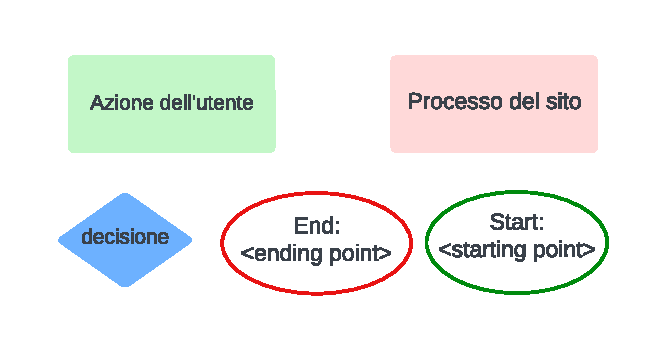
\includegraphics{materiale/uflegenda.pdf}
\end{center}
I punti di partenza (ellisse verde) e i punti di arrivo (ellisse rossa)
possono eventualmente specificare la pagina nella quale la task
termina.
\\\\
Si sottolinea che l'aspetto sequenziale degli user flows mostrato
nei diagrammi può essere interrotto, in ogni momento e pagina del
sito, da interazioni effettuate con la \textit{barra di navigazione}.
In particolare, dalla barra di navigazione è sempre possibile tornare
alla home page e al catalogo. Inoltre, la barra di navigazinoe può
adattarsi a seconda del livello di accesso dell'utente, aggiungendo
ulteriori interazioni possibili. Per semplificare i diagrammi ed
evitare eccessive ridondanze, le funzionalità della barra di navigazione
vengono descritte nella sezione dedicata al front-end.

\subsection{Registrazione e login}
\begin{figure}[H]
\centering
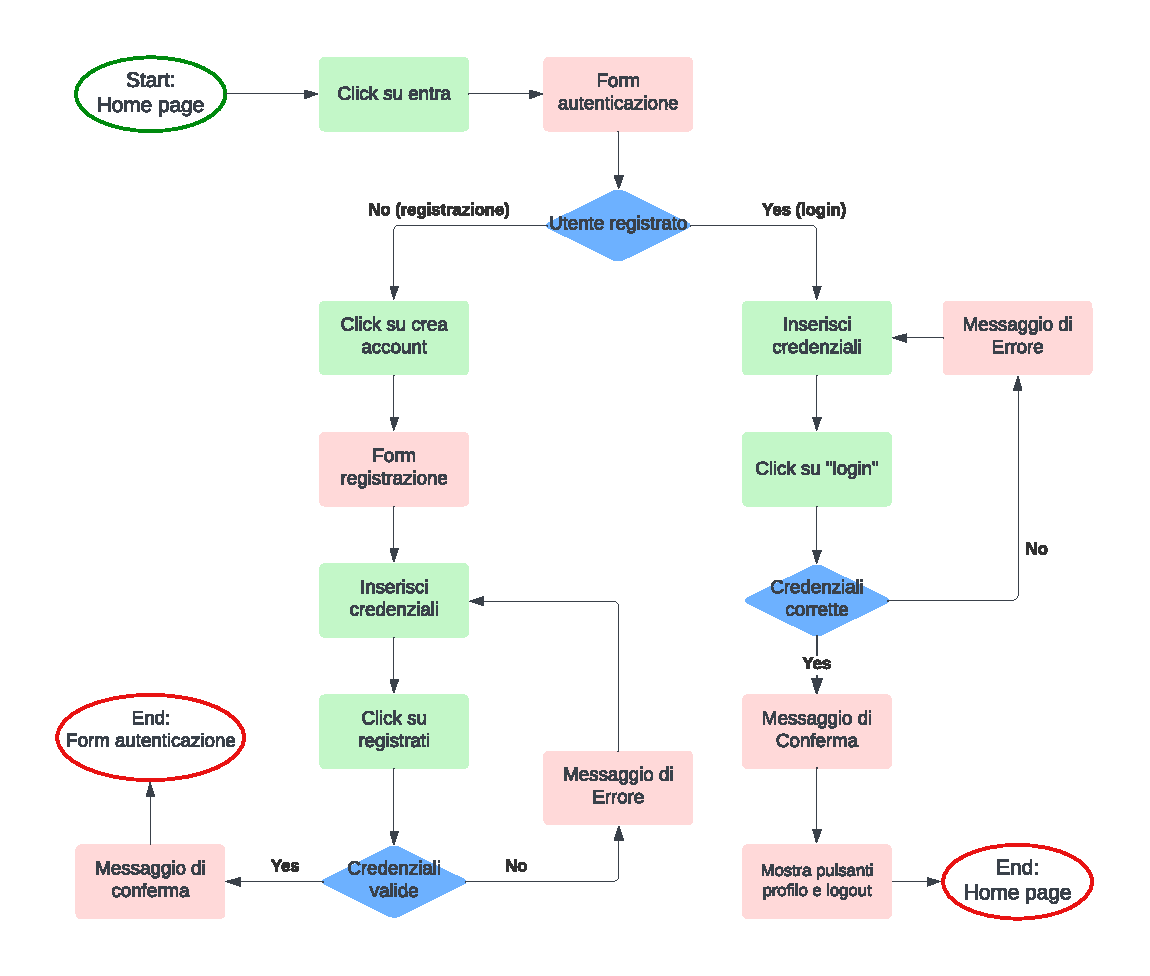
\includegraphics[width = \linewidth]{materiale/ufsignuplogin.pdf}
\end{figure}

\subsection{Risolvere un problema}
\begin{figure}[H]
\centering
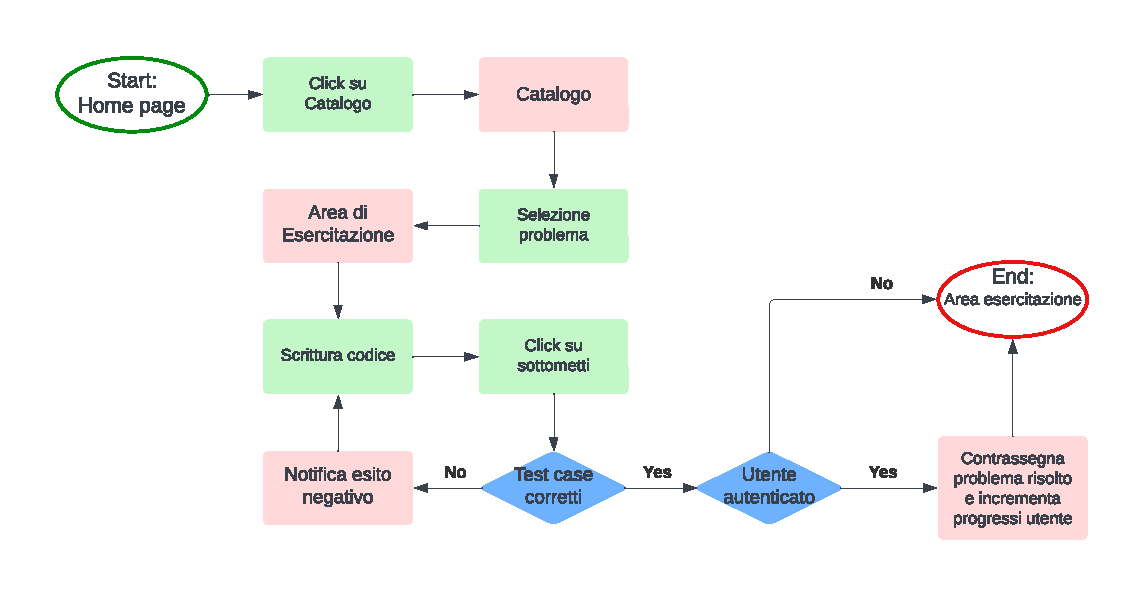
\includegraphics[width = \linewidth]{materiale/ufesercizio.pdf}
\end{figure}
  

\subsection{Gestire il profilo}
In questa sezione sono mostrati user flows legati alla gestione dei
dati personalizzabili dall'utente, principalmente legati all'account.

\subsubsection*{Modificare la password ed eliminare l'account}
Questi user flows mostrano rispettivamente come l'utente autenticato può modificare
la password e come può eliminare il proprio account.
\begin{figure}[H]
\centering
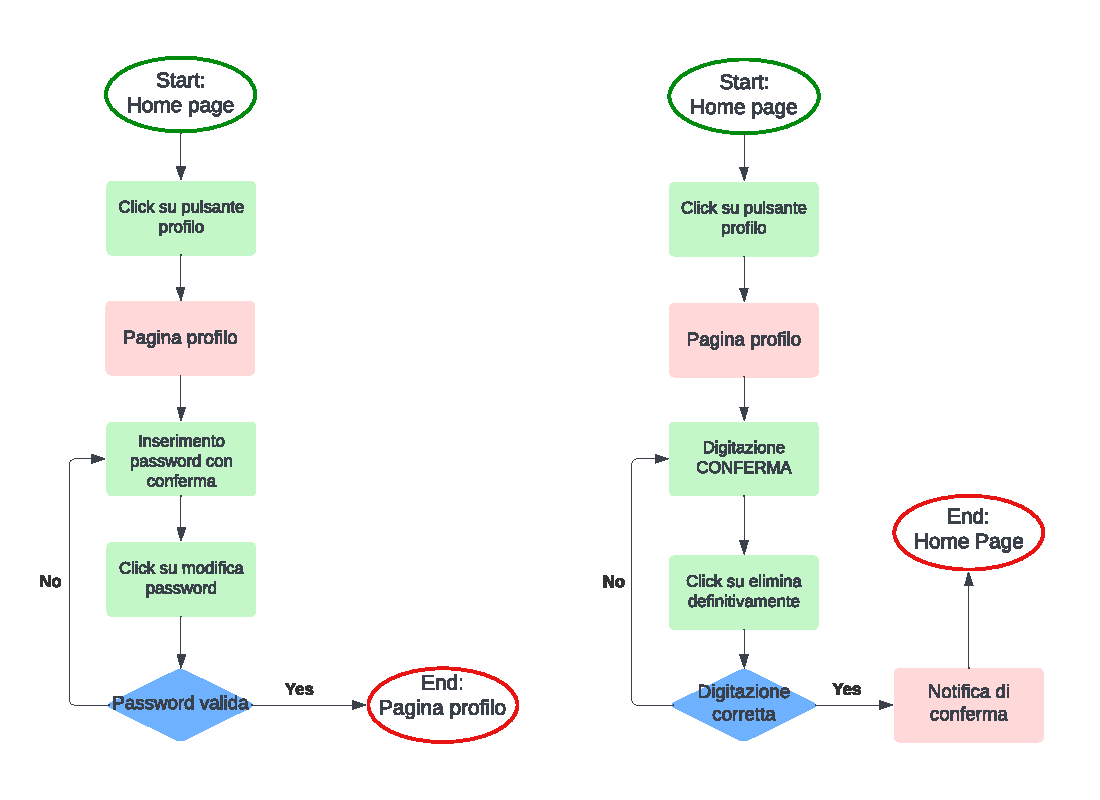
\includegraphics[width = \linewidth]{materiale/ufuserpage.pdf}
\end{figure}
Notare come, al termine dell'eliminazione dell'account, la piattaforma
reagisce conducendo l'utente alla home page.

\newpage\subsubsection*{Gestire i preferiti}
Questo user flow mostra come un utente può interagire con la piattaforma
al fine di modificare i problemi preferiti. Il diagramma distingue il
comportamento del flow a seconda del livello di accesso dell'utente.
\begin{figure}[H]
\centering
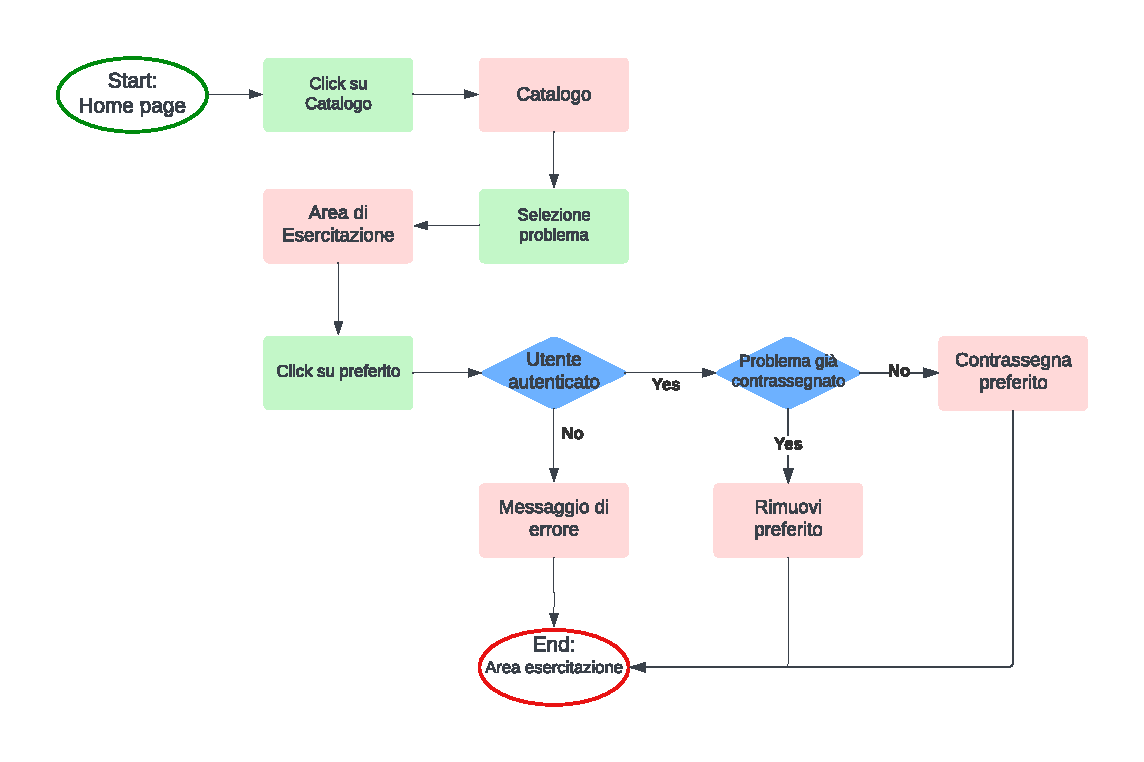
\includegraphics[width = \linewidth]{materiale/uflike.pdf}
\end{figure}
    

\subsection{Aggiungere un problema}
In questo user flow si assume che l'utente abbia i privilegi
del livello amministratore.
\begin{figure}[H]
\centering
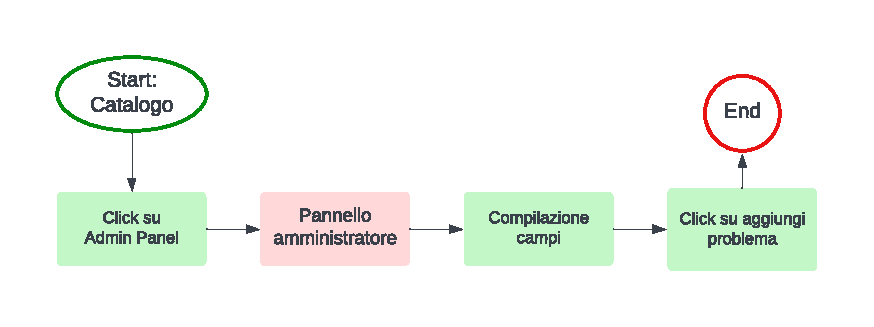
\includegraphics[width = \linewidth]{materiale/ufadmin.pdf}
\end{figure}
  

\newpage
\section{Documentazione e implementazione dell'applicazione}
Nella precedente sezione abbiamo illustrato tutte le funzioni attualmente implementate nell'applicazione e un'idea di come l'utente può interagire con esse.
L'applicazione SleepCode è stata sviluppata utilizzando \href{https://nextjs.org/}{Next.js} (versione 14.0.3), un framework Javascript free-open source basato su \href{https://react.dev/}{React}.

\subsection{Struttura del Progetto}
Il software utilizzato per il version control è \href{https://git-scm.com/}{Git}; come remote repository è stato impiegato \href{www.github.com}{GitHub},
il codice e la sua history è presente su una repository del membro del Team Raffaele Castagna, l'ultima versione stabile e quella utilizzata per hostare il sito è disponibile presso la repository CodeBase. All'interno della repository,
troveremo le seguenti cartelle:

\begin{figure}[H]
\centering
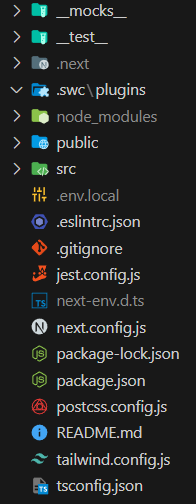
\includegraphics[scale = 1.2]{materiale/Project Structure.png}
\end{figure}

\noindent Ricordiamo che le cartelle \textbf{.next, .swc, .env} insieme a \textbf{package-lock.json, next-env.d.ts, eslintrc.json} sono state generate automaticamente.

\newpage
\subsubsection{Directory: \_\_mock\_\_ }
Questa cartella contine delle funzioni ``mock" che permettono a Jest di poter effetuare il testing senza fare chiamate dirette al database.
\subsubsection{Directory: \_\_test\_\_}
Questa cartella contiene tutti i test case e test suite dedicate al testing.
\subsubsection{Directory: public}
Questa cartella contiente tutte le immagini utilizzate all'interno del sito.
\subsubsection{Directory: src}
Questa cartella contiente tutte le parti del progetto sia front-end che back-end del progetto. Procediamo con una vista più dettagliata:

\begin{figure}[H]
  \centering
  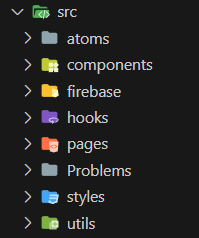
\includegraphics[scale = 1.2]{materiale/src.png}
\end{figure}

\begin{itemize}
  \item \textbf{Atoms}: È stata utilizzata una libreria di state management sviluppata da Google per tenere traccia dello stato dell'utente. La libreria utilizzata è: \href{https://recoiljs.org/}{Recoil}; gli atoms non sono altro che gli stati di certi componenti del sito.
  \item \textbf{Components}: Questa cartella contiene tutti i vari componenti del sito che vengono utilizzati dalle pagine, essi possono essere semplici \href{https://www.nngroup.com/articles/skeleton-screens/}{Scheletri} o componenti di maggior importanza.
  \item \textbf{Firebase}: Questa cartella contiene tutti i file relativi al setup di \href{https://firebase.google.com/}{Firebase}, il database utilizzato per il progetto.
  \item \textbf{Hooks}: Questa cartella contiene gli hooks sviluppati durante il progetto per compiere una funzione.
  \item \textbf{Pages}: Questa Cartella contiente le varie pagine le loro \textbf{routes} e le \textbf{API}.
  \item \textbf{Problems}: Questa cartella contiene il tipo di dato generico per i problemi.
  \item \textbf{Styles}: Questa cartella contiene diversi stili pre-impostati utilizzati assieme a \href{https://tailwindcss.com/}{TailwindCSS}.
  \item \textbf{Utils}: Questa cartella contiene i diversi testi e informazioni relative ai problemi attualmente disponibili, oltre che a form validators e funzioni comuni.
\end{itemize}

\subsubsection{.env.local}
Questa file contiene tutte le \textbf{variabili locali}, utilizzate per la connessione al database e necessarie per il corretto funzionamento dell'applicativo.
\subsubsection{.gitignore}
Questa cartella specifica quali file \textbf{git} non deve includere nelle varie pull/push requests. (.env.local è la più importante dal momento che essa contiente la \textbf{Chiave segreta}).
\subsubsection{jest.config.js}
Questo file contiene la configurazione di \textbf{Jest}, libreria utilizzata nel testing.
\subsubsection{package.json}
Questo file contiene le \textbf{dependencies} del framework.
\subsubsection{README.md}
Questo file contiene informazioni generali sul progetto.
\subsubsection{postcss.config.js}
Questo file è stato auto-generato da \href{https://tailwindcss.com/}{TailwindCSS}.
\subsubsection{tailwind.config.js}
Questo file contiene \textbf{palette} di colori utilizzati da \href{https://tailwindcss.com/}{TailwindCSS}.
\subsubsection{tsconfig.json}
Questo file contiene regole utilizzate da \href{https://eslint.org/}{ESLint} un \textbf{patter checker} utilizzato durante lo sviluppo.
  
\subsection{Dependencies del progetto}
Il progetto utilizza diverse librerie. Procediamo ad elencarne le più importanti e spiegare il loro funzionamento.
\begin{itemize}
  \item \href{https://codemirror.net/}{\textbf{CodeMirror}}: Utilizzata nel front-end, conferisce uno stile simile all'interfaccia grafica di VS Code durante la scrittura del codice.
  \item \href{https://split.js.org/}{\textbf{Split}}: Utilizzata nel front-end per rendere dinamica l'area di esercitazione (l'utente è in grado di modificare la grandezza dei componenti).
  \item \href{https://www.npmjs.com/package/react-toastify}{\textbf{Toastify}}: Libreria che offre componenti UI utilizzati per dialogare con l'utente.
  \item \href{https://recoiljs.org/}{\textbf{Recoil}}: Libreria di State Management sviluppata da Google.
  \item \href{https://firebase.google.com/docs/build}{\textbf{Librerie fornite da Firebase}}: Sono state impiegate diverse librerie fornite da Firebase come \textbf{auth, sdk, admin sdk} e molte altre.
  \item \href{https://www.npmjs.com/package/yup}{\textbf{Yup}}: Utilizzato per la validazione RegEx di dati inseriti.
  \item \href{https://eslint.org/}{\textbf{ESLint}}: Pattern checker utilizzato durante lo sviluppo per ottenere un codice di alta qualità.
  \item \href{https://jestjs.io/}{\textbf{Jest}}: Libreria utilizzata per il testing.
  \item \href{https://www.npmjs.com/package/node-mocks-http}{\textbf{node-mocks-http}}: Libreria utilizzata per mandare richieste API finte durante il testing.
\end{itemize}
%Oltre a queste abbia altre dipendenze minore tra vari \textbf{hooks} e pacchetti necessari per altri pacchetti inutili da elencare.

\newpage
\subsection{Dati del Progetti e Database}
Per il corretto funzionamento del sito, l'applicazione ha bisogno di consultare alcuni file locali. In seguito elencheremo alcune strutture dati utilizzate.
\subsubsection{Database}
Il database scelto per memorizzare i dati è \href{https://firebase.google.com}{\textbf{Firebase}}, per essere più specifici \textbf{Firestore}, il sottoinsieme che si occupa della memorizazzione dei dati in cloud.
Sono state individuate due collezioni da dover inserire nel database e due collezioni da tenere in locale per facilitare lo sviluppo così da poter operare in maniera ``strict''.

\subsubsection*{Problem}
Questo modello rappresenta un problema generico all'interno dell'applicazione, ciò che l'applicazione sa su un problema è differente da ciò che il database memorizza; questo è dovuto sia per motivi di semplicità che limiti sui dati che possiamo mantenere nel cloud.
Ci sono alcuni campi la cui funzione non è immediatiamente chiara, quindi verrà descritta la funzione di ogni campo.  

\begin{itemize}
  \item \textbf{id}: l'id del problema, per semplicità l'id dei problemi è il loro titolo in minuscolo con "-" al posto degli spazi.
  \item \textbf{title}: Il nome del problema.
  \item \textbf{problemStatement}: La descrizione del problema.
  \item \textbf{examples}: Contiente tutti gli esempi da mostrare all'utente.
  \item \textbf{constraints}: Nel caso gli input e/o output abbiano certe regole da rispettare questa campo le conterrà.
  \item \textbf{order}: Ad ogni problema assegneremo un numero che verrà utilizzato nell'ordinamento dei problema nella pagina principale.
  \item \textbf{starterCode}: Le linee di testo presenti appena si apre un problema per la prima volta.
  \item \textbf{handlerFunction}: Funzione associata ad ogni problema che permette la sottomissione e il controllo del codice scritto dall'utente.
  \item \textbf{starterFunctionName}: Nome della funzione associata al problema.
\end{itemize}

\begin{figure}[H]
  \centering
  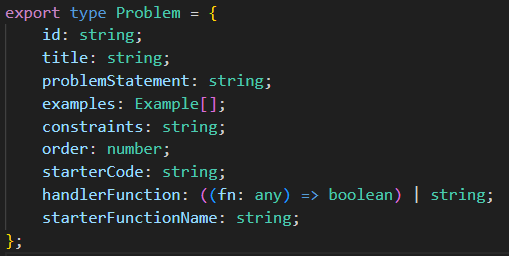
\includegraphics[width=10cm]{materiale/Problem Template.png}
\end{figure}

\subsubsection*{Example}
Questo modello indica come deve essere strutturato un esempio all'interno del problema. Esso include due campi opzionali (\textbf{explanation, img}) che possono non essere presenti in alcuni problemi.
\begin{figure}[H]
  \centering
  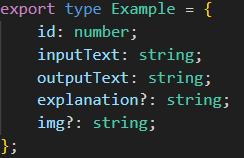
\includegraphics[width=5cm]{materiale/Example Template.png}  
\end{figure}

\subsubsection*{DBProblem}
Questo modello rappresenta i dati che vengono raccolti dal database riguardanti ogni problema. Anche qui abbiamo un campo opzionale \textbf{videoId}.
\begin{figure}[H]
  \centering
  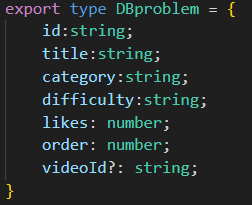
\includegraphics[width=5cm]{materiale/DBProblem Template.png}
\end{figure}

\subsubsection*{userData}
Questo Modello rappresenta i dati che riguardano ogni utente al momento della registrazione. Il ruolo di ``\textbf{User}" viene assegnato inizialmente ad ogni utente e successivamente attraverso console di Firestore verrà cambiato manualmente a ``\textbf{Administrator}"
se si intende promuovere l'utente al livello di amministratore.

\begin{figure}[H]
  \centering
  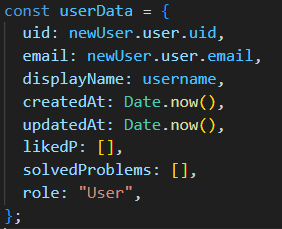
\includegraphics[width=5cm]{materiale/User Template.png}
\end{figure}


\subsection{Project API}
In questa parte del documento sono presentate le API dell'applicazione SleepCode.
Esse saranno prima descritte e, successivamente, verrà mostrato il loro codice.

\subsubsection{Estrazione delle risorse dal class diagram}
Analizzando il diagramma delle classi sono state individuate due risorse principali: l'utente e i problemi. Di seguito riportiamo le API:

\subsubsection{API riguardanti l'utente}
\begin{itemize}
  \item \textbf{signUp (\texttt{POST})}: Questa API permette all'utente non ancora autenticato di creare un account sulla piattaforma per tracciare i progressi e i preferiti. Se tutte le informazioni sono valide, l'account verrà creato normalmente, altrimenti l'utente riceverà una notifica di errore.
  \item \textbf{deleteAccount (\texttt{DELETE})}: Questa API permette all'utente autenticato di eliminare il proprio account e tutte le informazioni associate ad esso. (I \textit{preferiti} contrassegnati dall'utente e collezionati dai problemi rimarrano nel database in modo da avere uno storico dei problemi, e il loro ammontare di ``likes'', più accurato).
  \item \textbf{changePassword (\texttt{PATCH})}: Questa API permette all'utente autenticato di poter cambiare la propria password, effettuando tale operazione sul sito stesso. Se le informazioni sono valide, la password verrà cambiata, altrimenti l'utente riceverà una notifica di errore.
\end{itemize}

\subsubsection{API riguardanti i problemi}
\begin{itemize}
  \item \textbf{getProblems (\texttt{GET})}: Questa API viene chiamata quando un utente (autenticato o non) si connette alla pagina del catalogo. Essa ritorna la lista di problemi disponibili in quel momento.
\end{itemize}

\begin{figure}[H]
  \hspace*{-2cm}
  \centering
  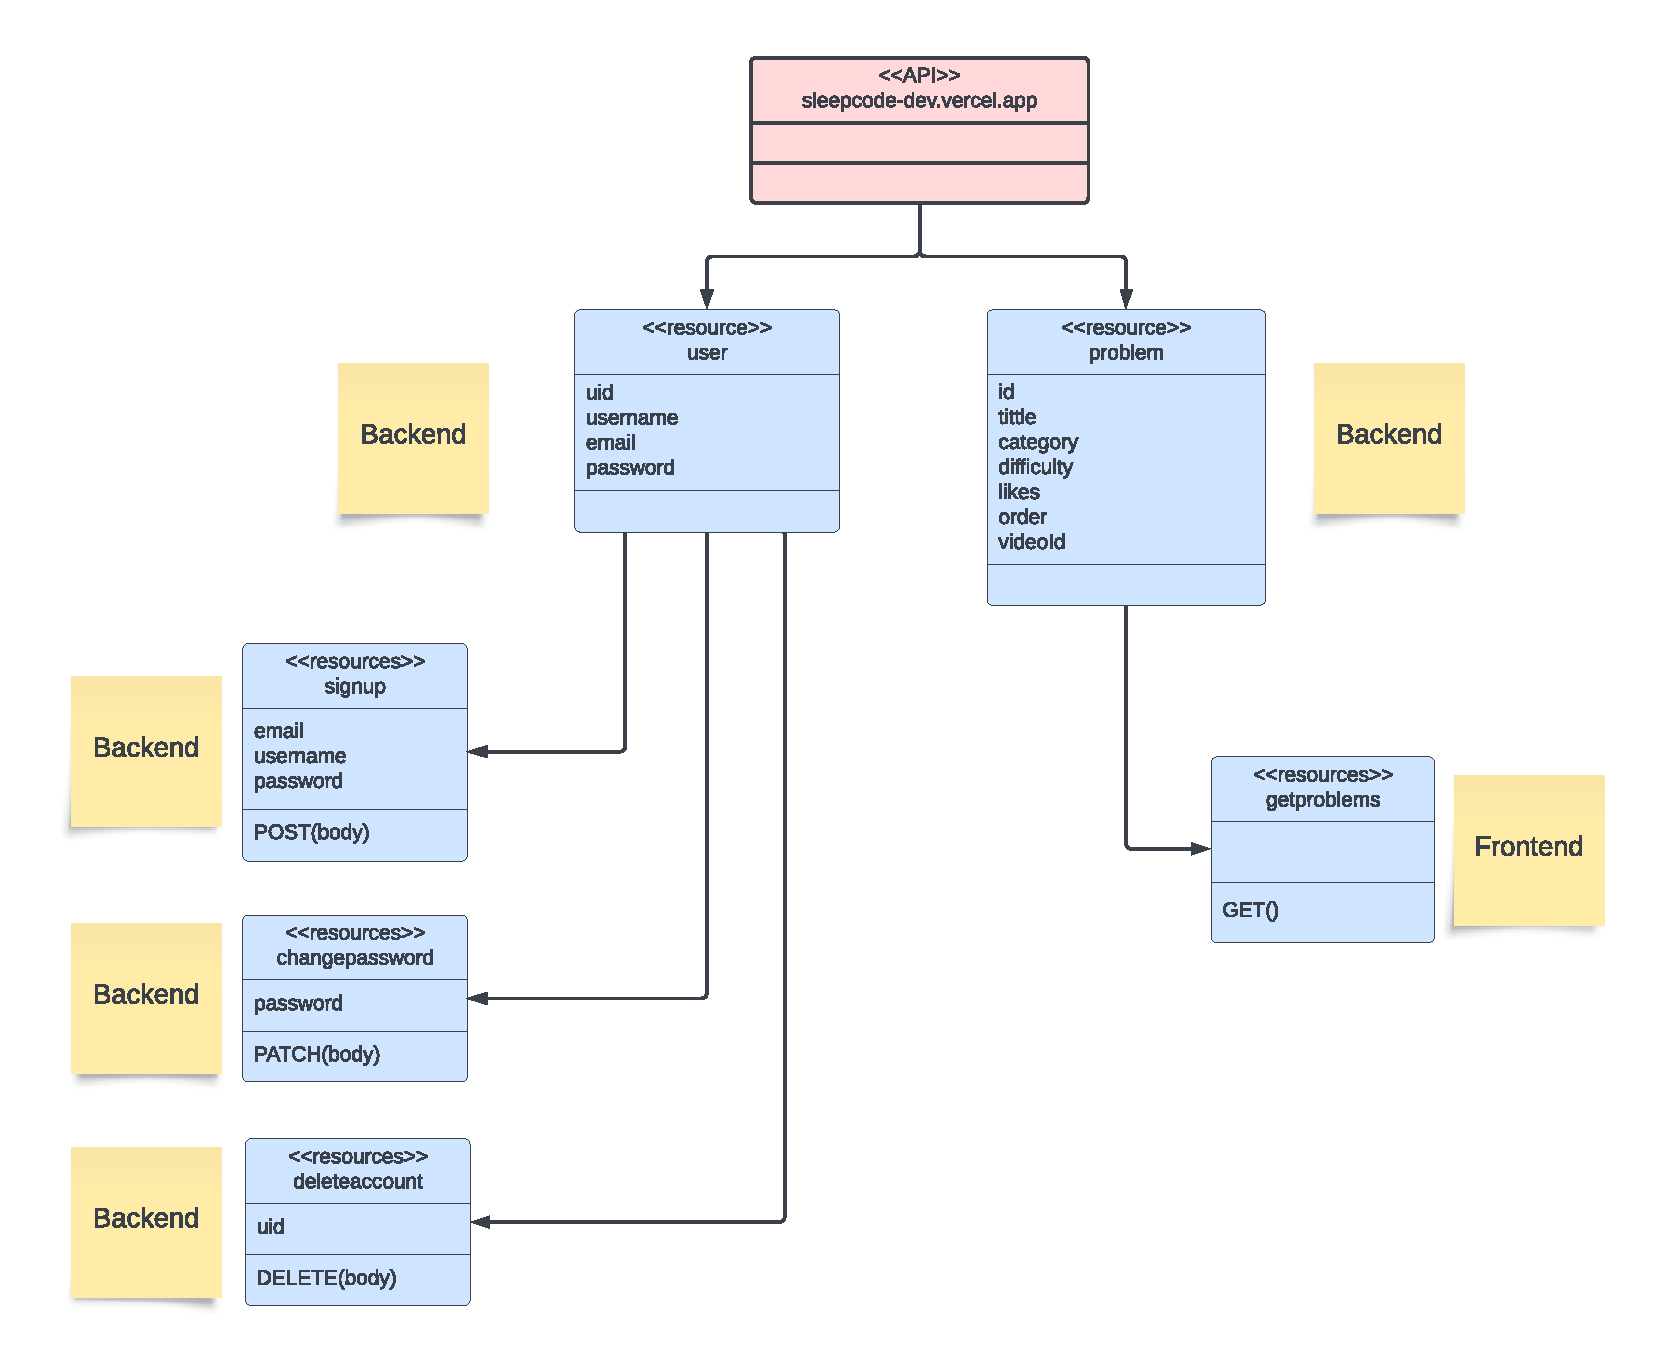
\includegraphics[scale = 0.6]{materiale/Resource diagram.pdf}
\end{figure}

\subsubsection{Resource Models}
Il Resource model esprime, per ogni API, le diverse risposte, come le richieste sono strutturate e come ci si può accedere.
Ogni API dovrà elaborare il body (se lo richiede), ovvero le informazioni necessarie per il corretto funzionamento, e risponderà appropriatamente con uno \href{https://developer.mozilla.org/en-US/docs/Web/HTTP/Status}{Status Code}.
Il body viene rappresentato tramite una freccia che uscente e le risposte sono rappresentate tramite delle freccie entranti.

\subsubsection*{User API}
\begin{figure}[H]
  \hspace*{-2.4cm}
  \centering
  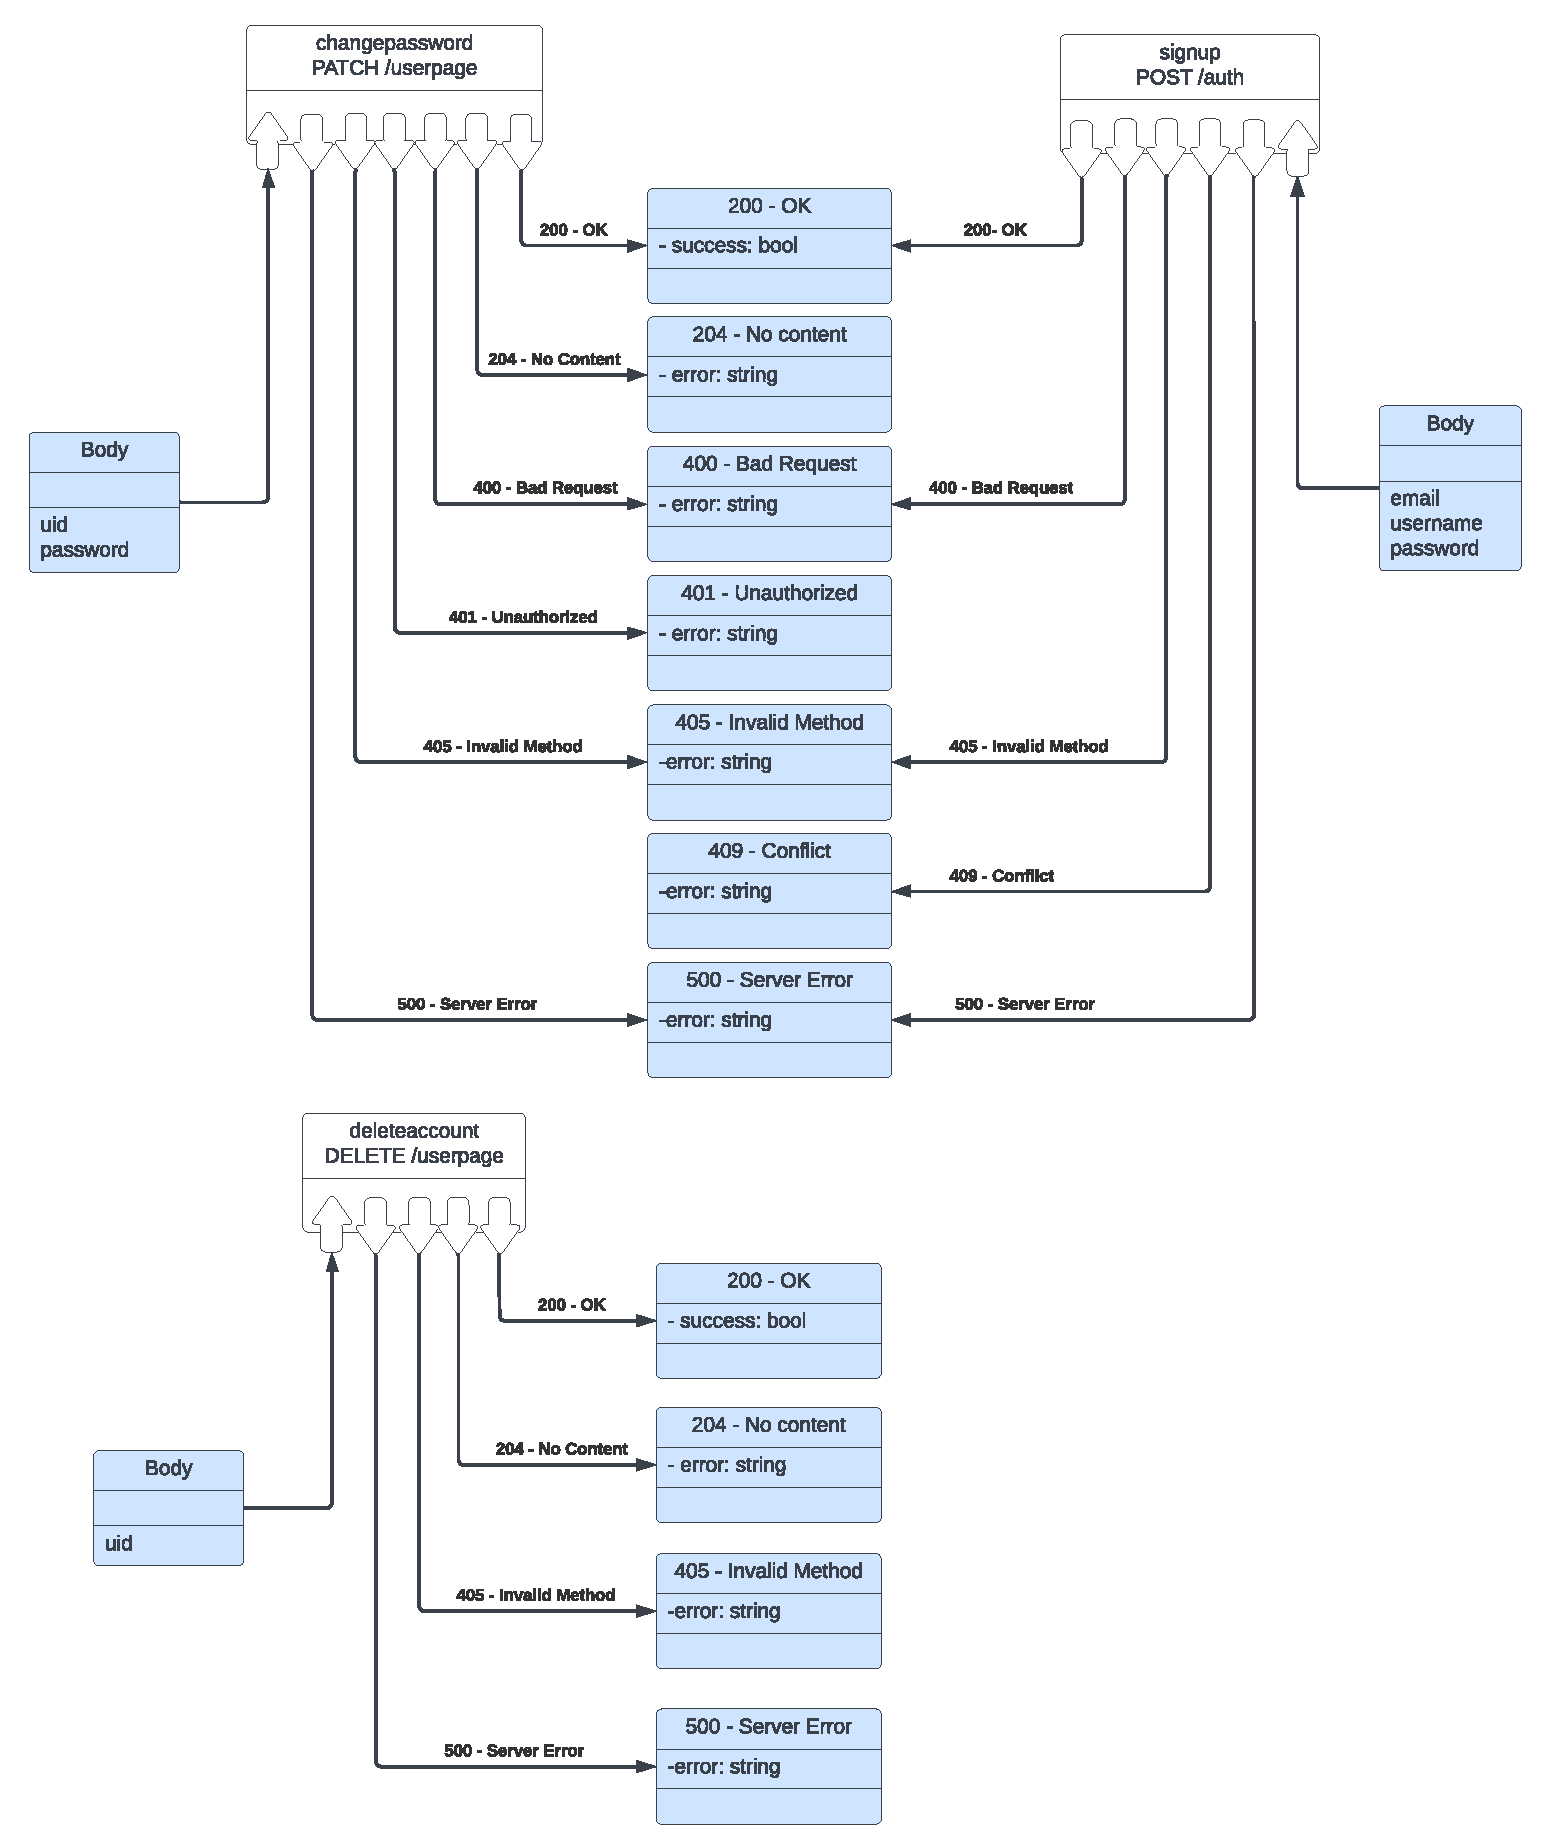
\includegraphics[scale = 0.64]{materiale/Resource Models Users.pdf}
\end{figure}

\newpage
\textbullet \textbf{ Problem API}\\
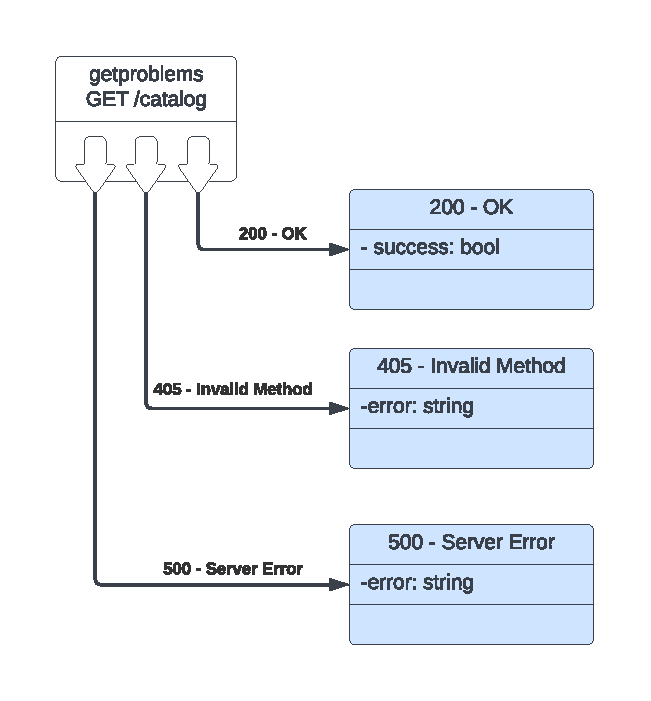
\includegraphics[width=\textwidth]{materiale/Resource Models Problems.pdf}

\newpage
\subsection{Sviluppo API}
In questa sezione mostreremo il codice relativo alle API.
\subsubsection{Signup}
\begin{figure}[H]
  \centering
  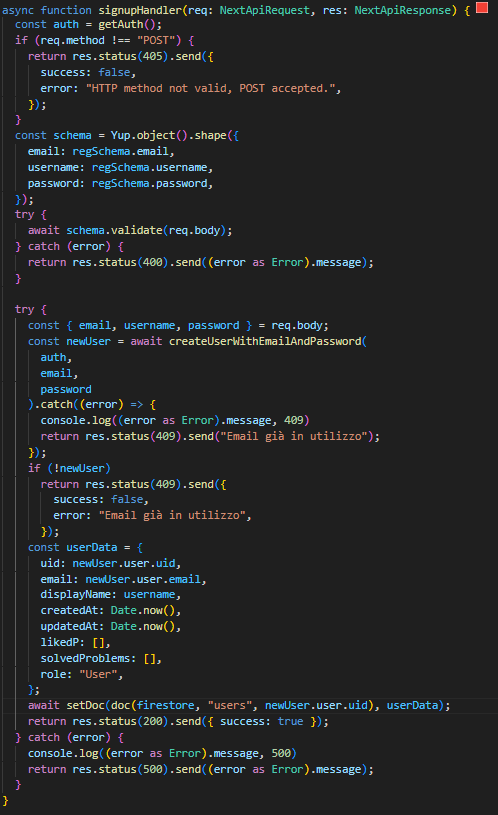
\includegraphics[scale = 0.8]{materiale/API/signup.png}
\end{figure}

Questa API permette ad un utente di registrarsi all'interno dell'applicazione: essa richiede un'email, un username e una password.
Attraverso la libreria Yup viene verificato che le informazioni inserite dall'utente siano accettabili; se accettabili, il sistema proverà a registrare l'utente.
In caso vi siano problemi di conflitto nella creazione dell'utente, l'HTTP response avrà Status Code 409; in caso di una password e/o username malformati avremo uno Status code 400;
in caso di un qualsiasi errore non precedentemente previsto avremo HTTP 500; in caso la richiesta è malformata avremo HTTP 405 e in caso di successo HTTP 200.

\subsubsection{deleteAccount}
\begin{figure}[H]
  \centering
  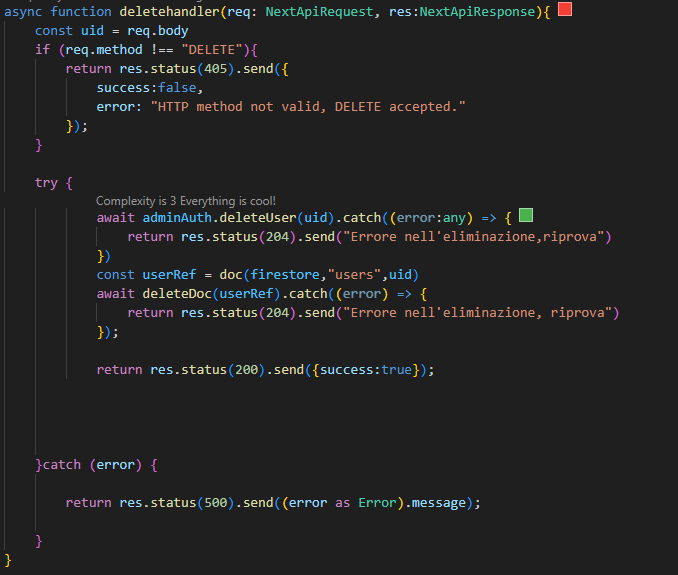
\includegraphics[width=\textwidth]{materiale/API/deleteAccount.png}  
\end{figure}

Questa API permette ad un utente autenticato di eliminare il proprio account e tutti i dati relativi ad esso (ricordiamo che per avere uno storico più accurato i like non verrano rimossi dai problemi),dopo che la richiesta
è stata ricevuta elimineremo prima l'account dell'utente e successivamente tutti i dati contenuti nel database.
In caso la richiesta sia malformata avremo HTTP 405, in caso di problemi (come utente inesistente e/o già eliminato) avremo HTTP 204,in caso di problemi col server avremo HTTP 500, e in caso di successo HTTP 200

\subsubsection{changePassword}
\begin{figure}[H]
  \centering
  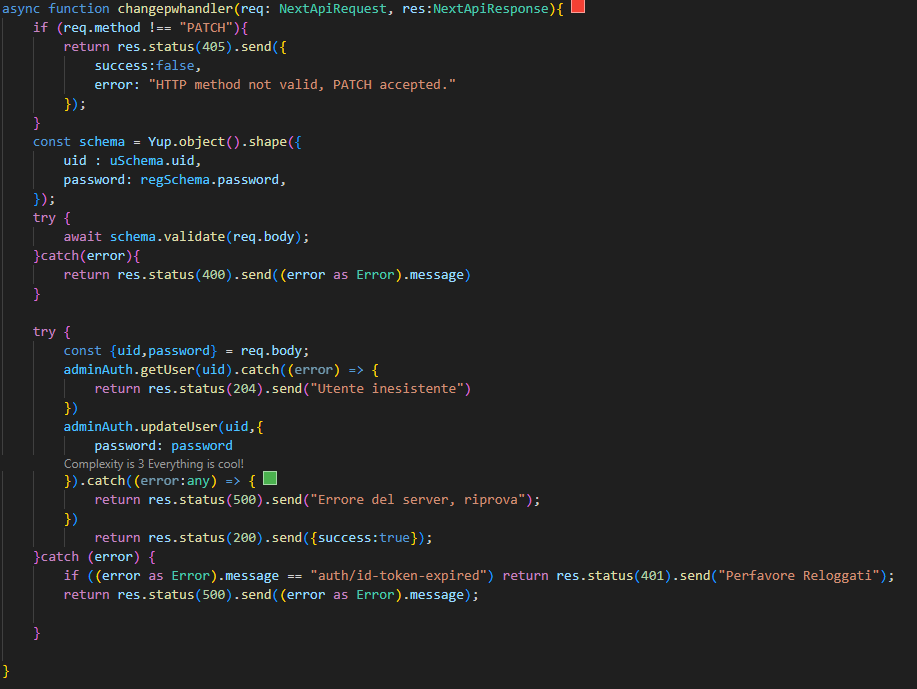
\includegraphics[width=\textwidth]{materiale/API/ChangePassword.png}  
\end{figure}
Questa API permette all'utente di modificare la propria password, sempre che rispetti i requisiti per essere una password forte.
Dopo aver ricevuto una richiesta, si controllerà che la password rispetti i requisiti per essere tale, dopodichè verrà controllata l'esistenza
dell'utente e, se esso esiste, la password verrà cambiata con quella appena fornita.
In caso la richiesta sia malformata, lo status code sarà HTTP 405, in caso la password fornita sia malformata avremp HTTP 400, in caso di utente inesistente HTTP 204,
in caso qualcosa vada storto con l'operazione di modifica, per altre ragioni,
lo status code corrisponderà a HTTP 500, e in caso di successo HTTP 200.

\subsubsection{getProblems}
\begin{figure}[H]
  \centering
  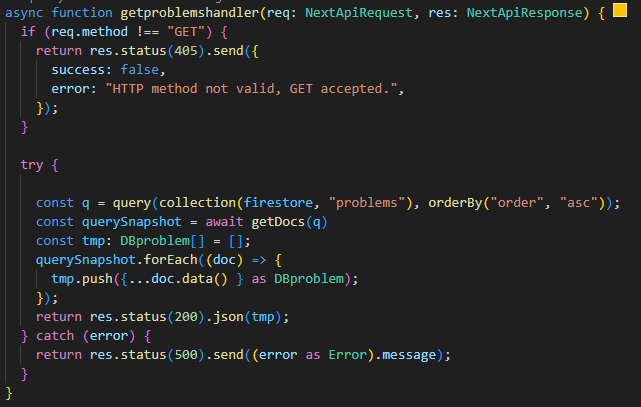
\includegraphics[width=\textwidth]{materiale/API/GetProblems.png}
\end{figure}
Questa API resistuisce i problemi disponibili al momento della richiesta e tutti i dati relativi ad essi (ordine, titolo, difficoltà, videoId, categoria ecc).
Dopo aver ricevuto una richiesta, una query verrà inviata al Firestore per ottenere i dati relativi a tutti i problemi presenti nella collection problems.
In caso la richiesta sia malformata lo status code sarà HTTP 405, in caso la richiesta incontri qualsiasi problema durante la query HTTP 500, in caso di successo HTTP 200.
\newpage
\subsection{Documentazione API}
Le API fornite dall'applicativo, presentate nella sezione precedente, sono state documente utilizzando il pacchetto NPM \href{https://www.npmjs.com/package/swagger}{Swagger},
Grazie a questo pacchetto, è stato possibile generare una pagina web dedicata alla definizione delle specifiche OpenAPI (Figura \ref{documentazione}), la quale è disponibile attraverso questo link: \href{https://sleepcode-dev.vercel.app/api-doc}{api-doc}.
La documentazione è reperibile anche nel codice sorgente.

Durante lo sviluppo delle API sono stati impiegati diversi metodi:
\begin{itemize}
  \item \texttt{GET}: utilizzato per ottenere dati da un server, non contiene body.
  \item \texttt{POST}: utilizzato per creare risorse su un server.
  \item \texttt{PATCH}: utilizzato per modificare una risorsa su un server.
  \item \texttt{DELETE}: utilizzato per eliminare risorse da un server.
\end{itemize}

\begin{figure}[H]
  \centering
  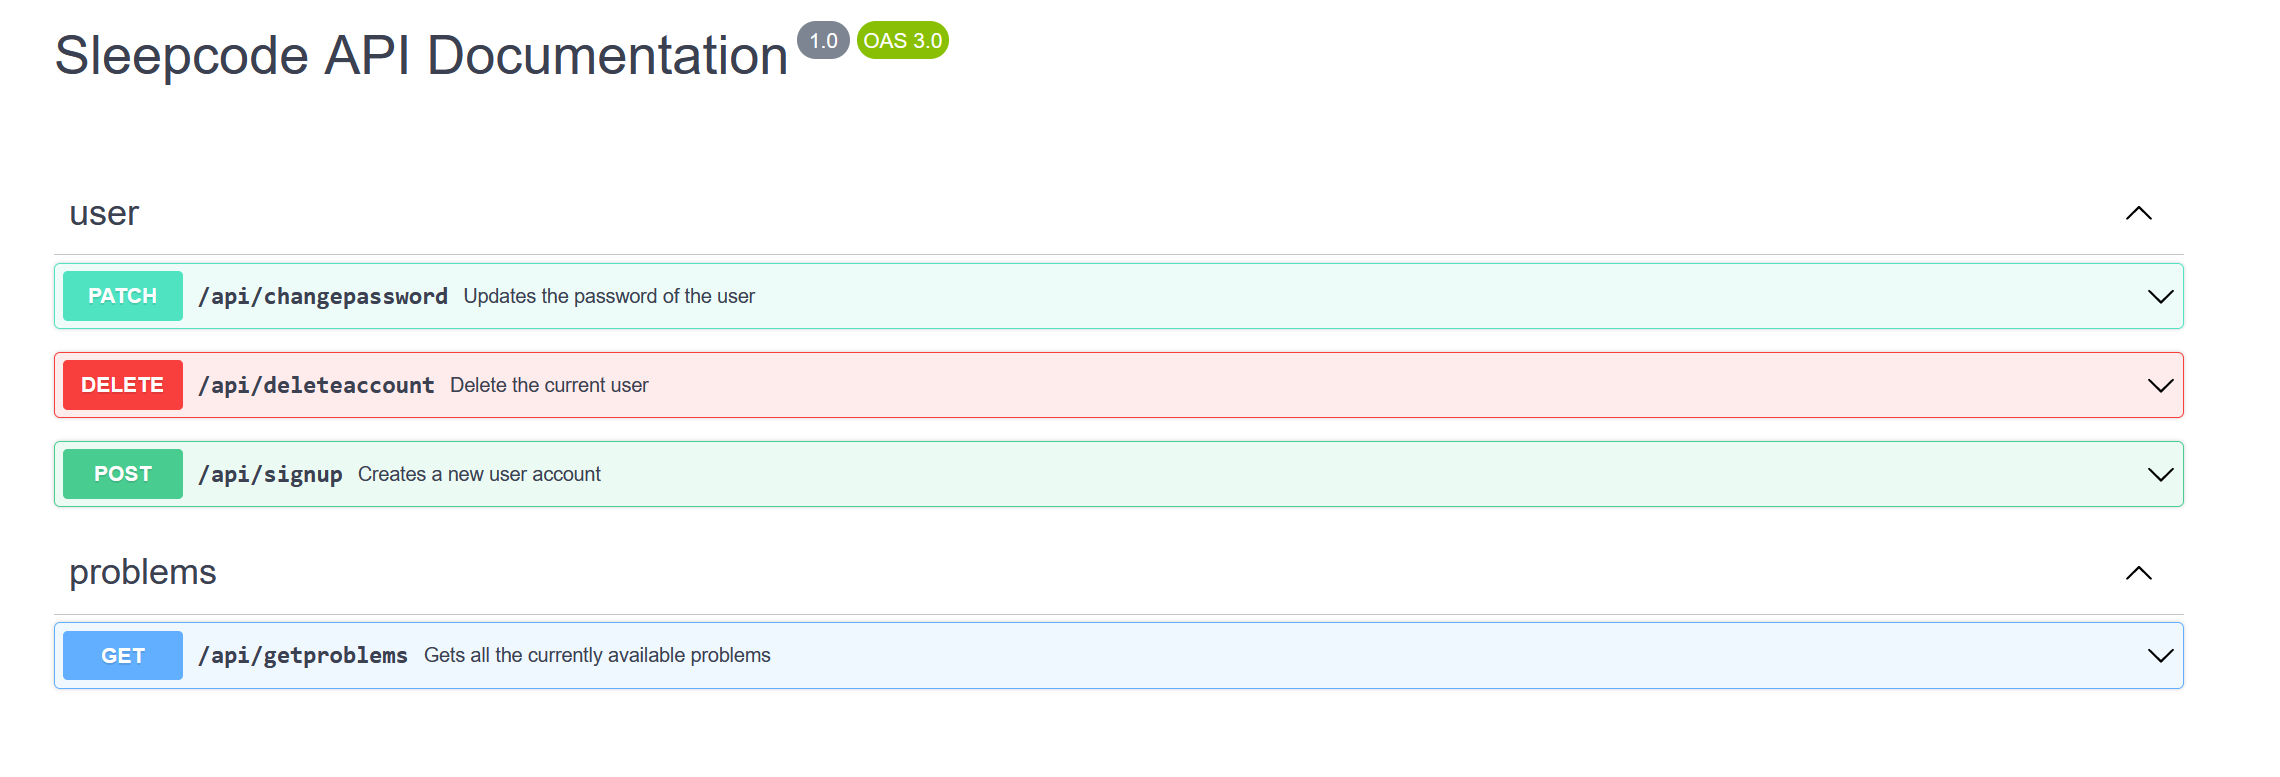
\includegraphics[width=\textwidth]{materiale/API/API-doc.png}
  \caption{Un'immagine che mostra la pagina contenente la documentazione}
  \label{documentazione}
\end{figure}

\newpage
\section{Frontend}
In questa sezione del documento verrà mostrata una parte vitale dell'applicazione: il \textbf{front-end}, ovvero la parte dell'applicazione con cui l'utente finale interagisce.
Per ogni componente viene fornita una breve descrizione delle azioni disponibili all'utente.

\subsection{Home}
La Home è la prima schermata che un utente vede appena si connette al sito. Essa contiene una NavBar (presente in ogni pagina) che contiente diversi bottoni:
\begin{itemize}
  \item Home: Questo bottone, se cliccato, riporterà l'utente alla pagina principale.
  \item Catalogo: Questo bottone, se cliccato, porterà l'utente alla pagina del catalogo contente tutti i problemi.
  \item Admin Panel: Questo bottone appare solo se nel Database l'utente ha come ruolo ``Administrator". Eicordiamo che il ruolo di ogni utente è ``User" e per promuovere un utente
  si dovrà interagire con la \textbf{CLI} di Firebase per modificare il ruolo del singolo utente. Questo può essere fatto solo da persone connesse al progetto sul sito di Firebase.
  \item Pagina Profilo: Questo Bottone appare solo se l'utente è autenticato. Se si posiziona il cursore del mouse al di sopra, verrà visualizzata l'email dell'utente attualmente collegato; se cliccato, si arriverà alla pagina del profilo utente.
  \item Bottone di Login: Questo bottone compare solo se l'utente non è attualmente autenticato; ha lo scopo di aprire il form di login.
  \item Bottone di Logout: Questo bottone compare solo se l'utente è autenticato, e se cliccato effettua l'operazione di logout.
\end{itemize}

\begin{figure}[H]
  \centering
  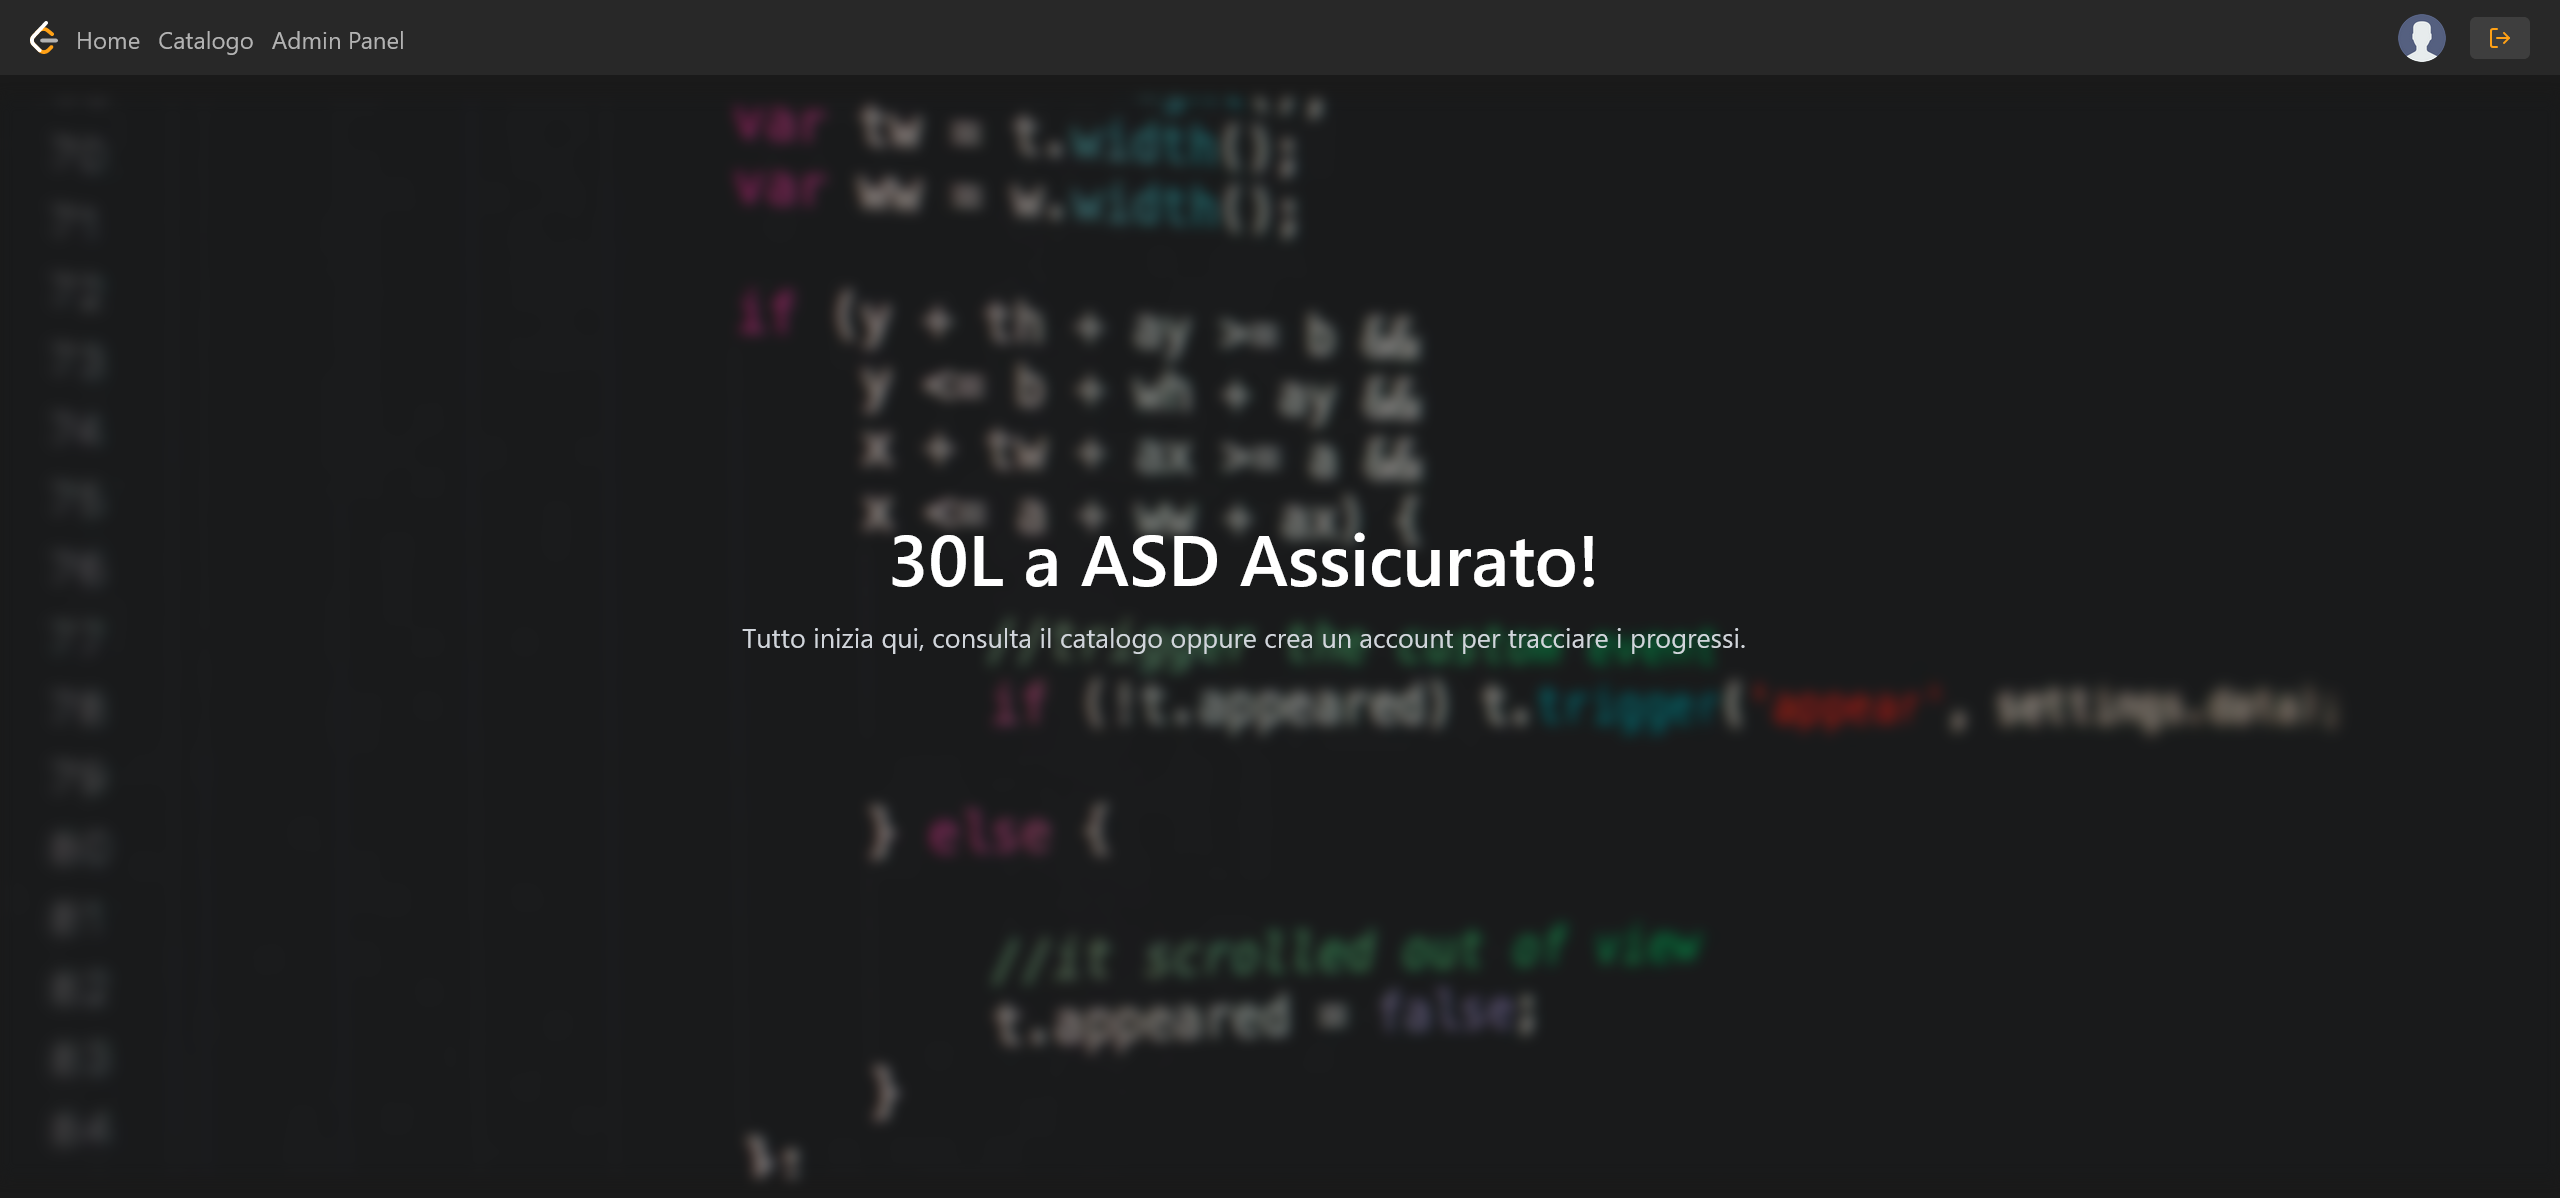
\includegraphics[width=\textwidth]{materiale/sito/Home.png}
\end{figure}

\subsection{Login}
Questo componente permette ad un utente non ancora autenticato ma registrato di entrare con le proprie credenziali\footnote{A causa di regole imposte da firebase e non modificabili,
la password che viene data non viene controllata se conforme dato che il modello
di recupero password di Firebase non permette l'impostazione di regole per la password strength nel piano gratuito}.
Se l'utente ha inserito le proprie credenziali e sono corrette allora verrà autenticato con messaggio di conferma,
altrimenti avrà un messaggio di errore.

\begin{figure}[H]
  \centering
  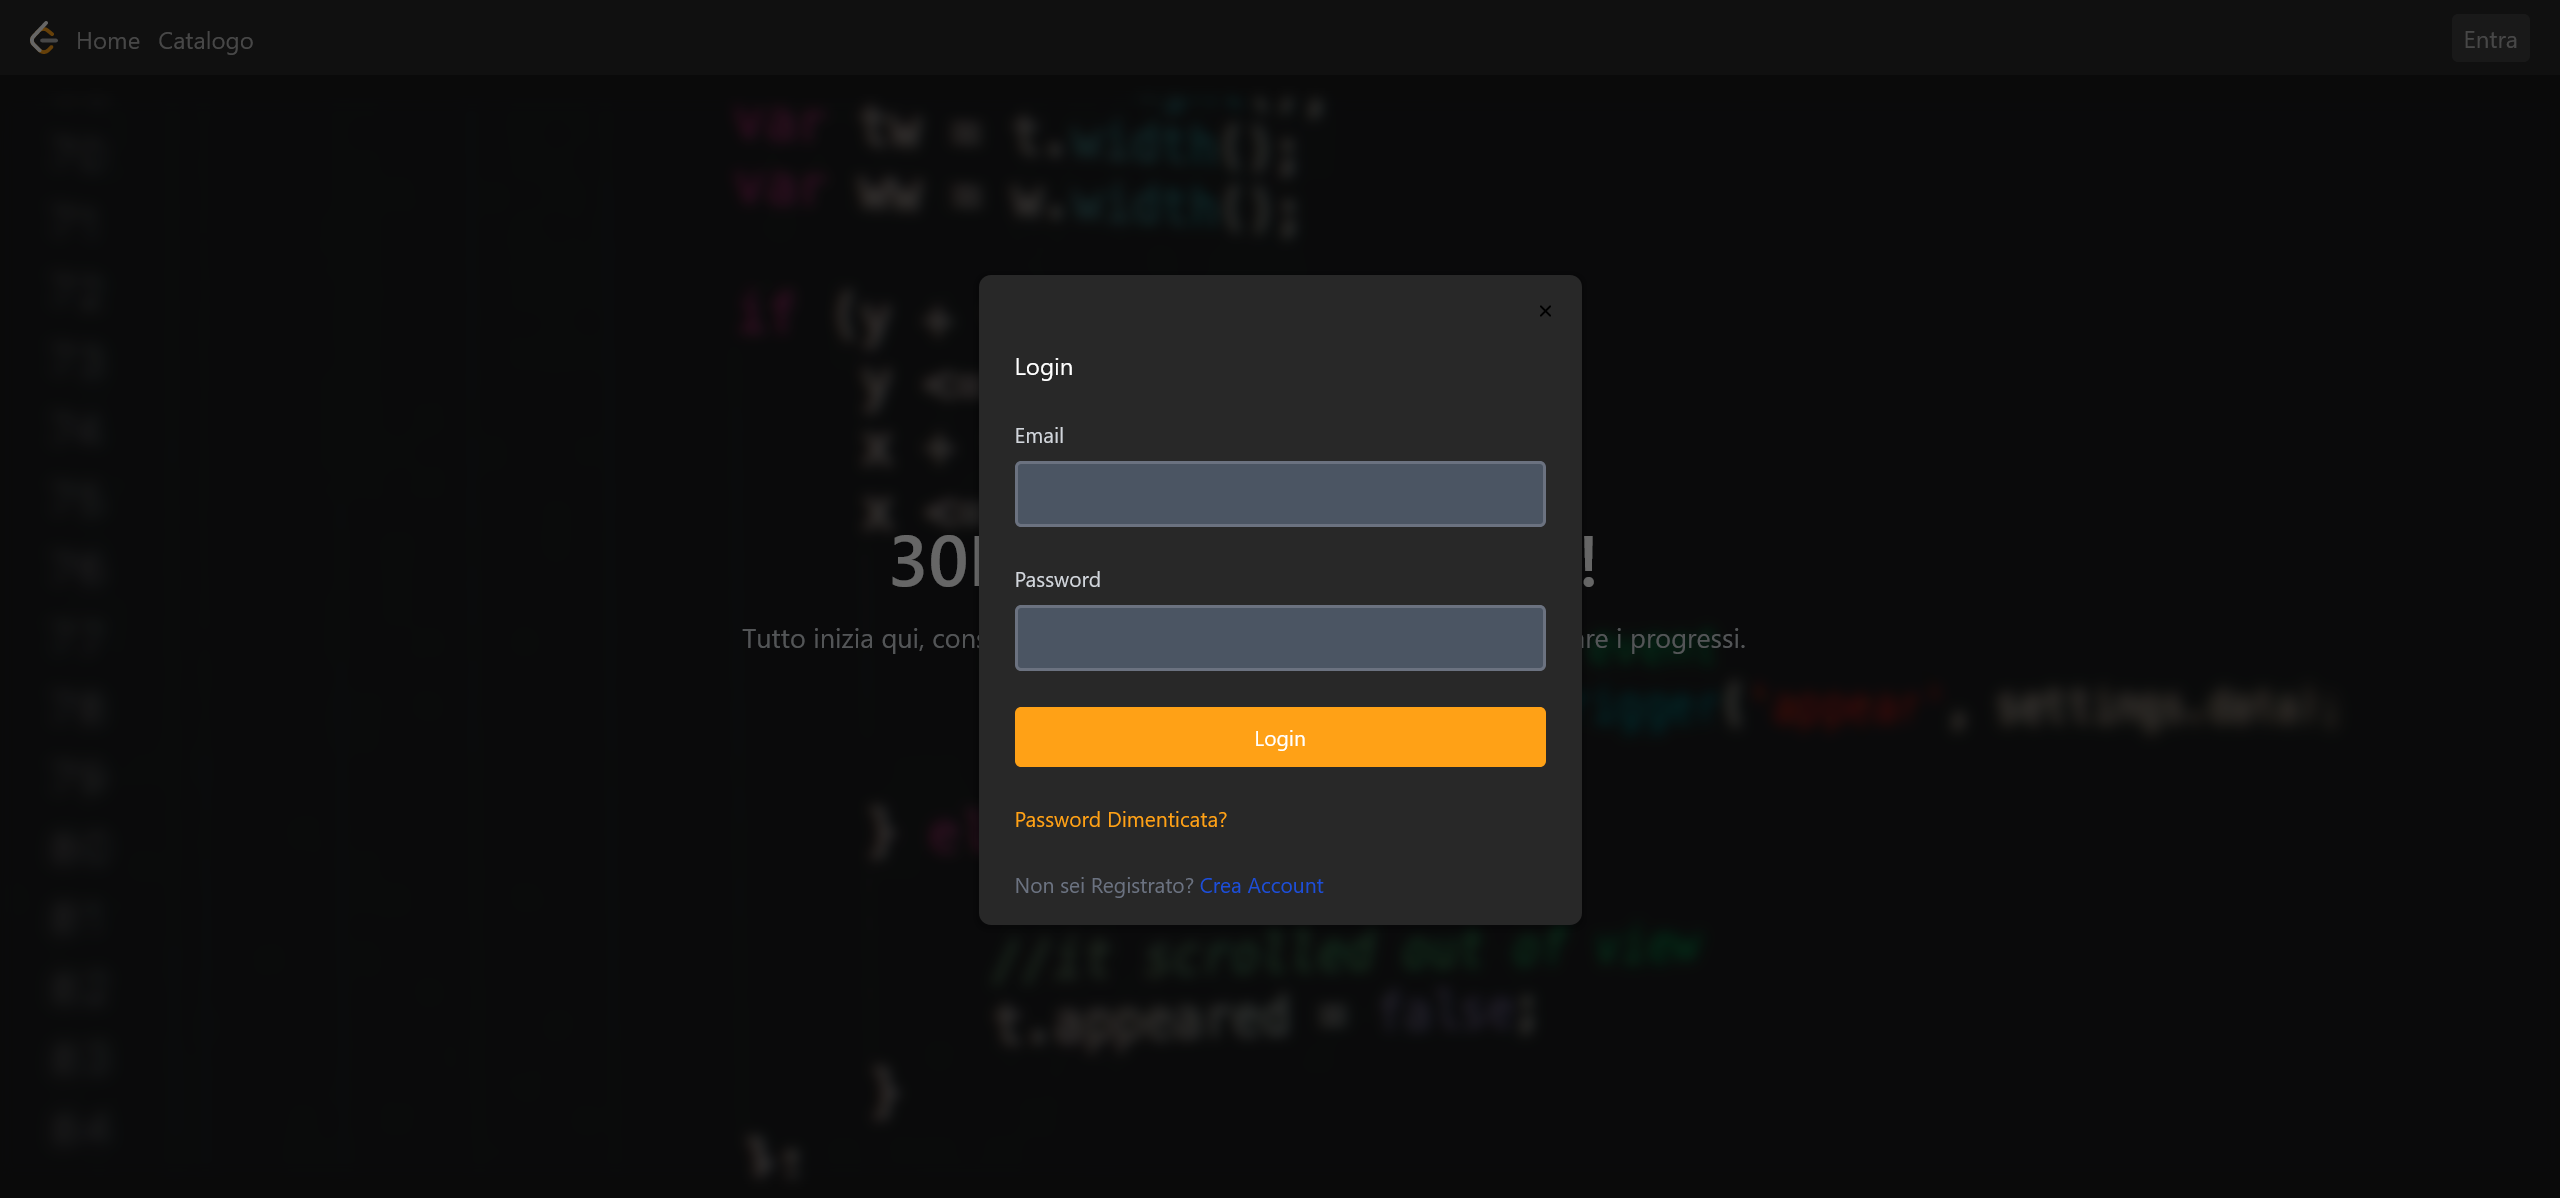
\includegraphics[width=\textwidth]{materiale/sito/Login.png}
\end{figure}

\subsection{Signup}
Questo componente permette ad un utente non ancora autenticato di registrarsi, l'utente dovrà fornire un'email,username e password, username e password verrano controllati attraverso \textbf{Yup} se rispettano i criteri imposti, in caso contrario l'utente verrà avvertito tramite messagio di errore.
In caso i dati inseriti sono corretti allora l'utente verrà rimandato al componente di Login con messaggio di successo.\\\\

\begin{figure}[H]
  \centering
  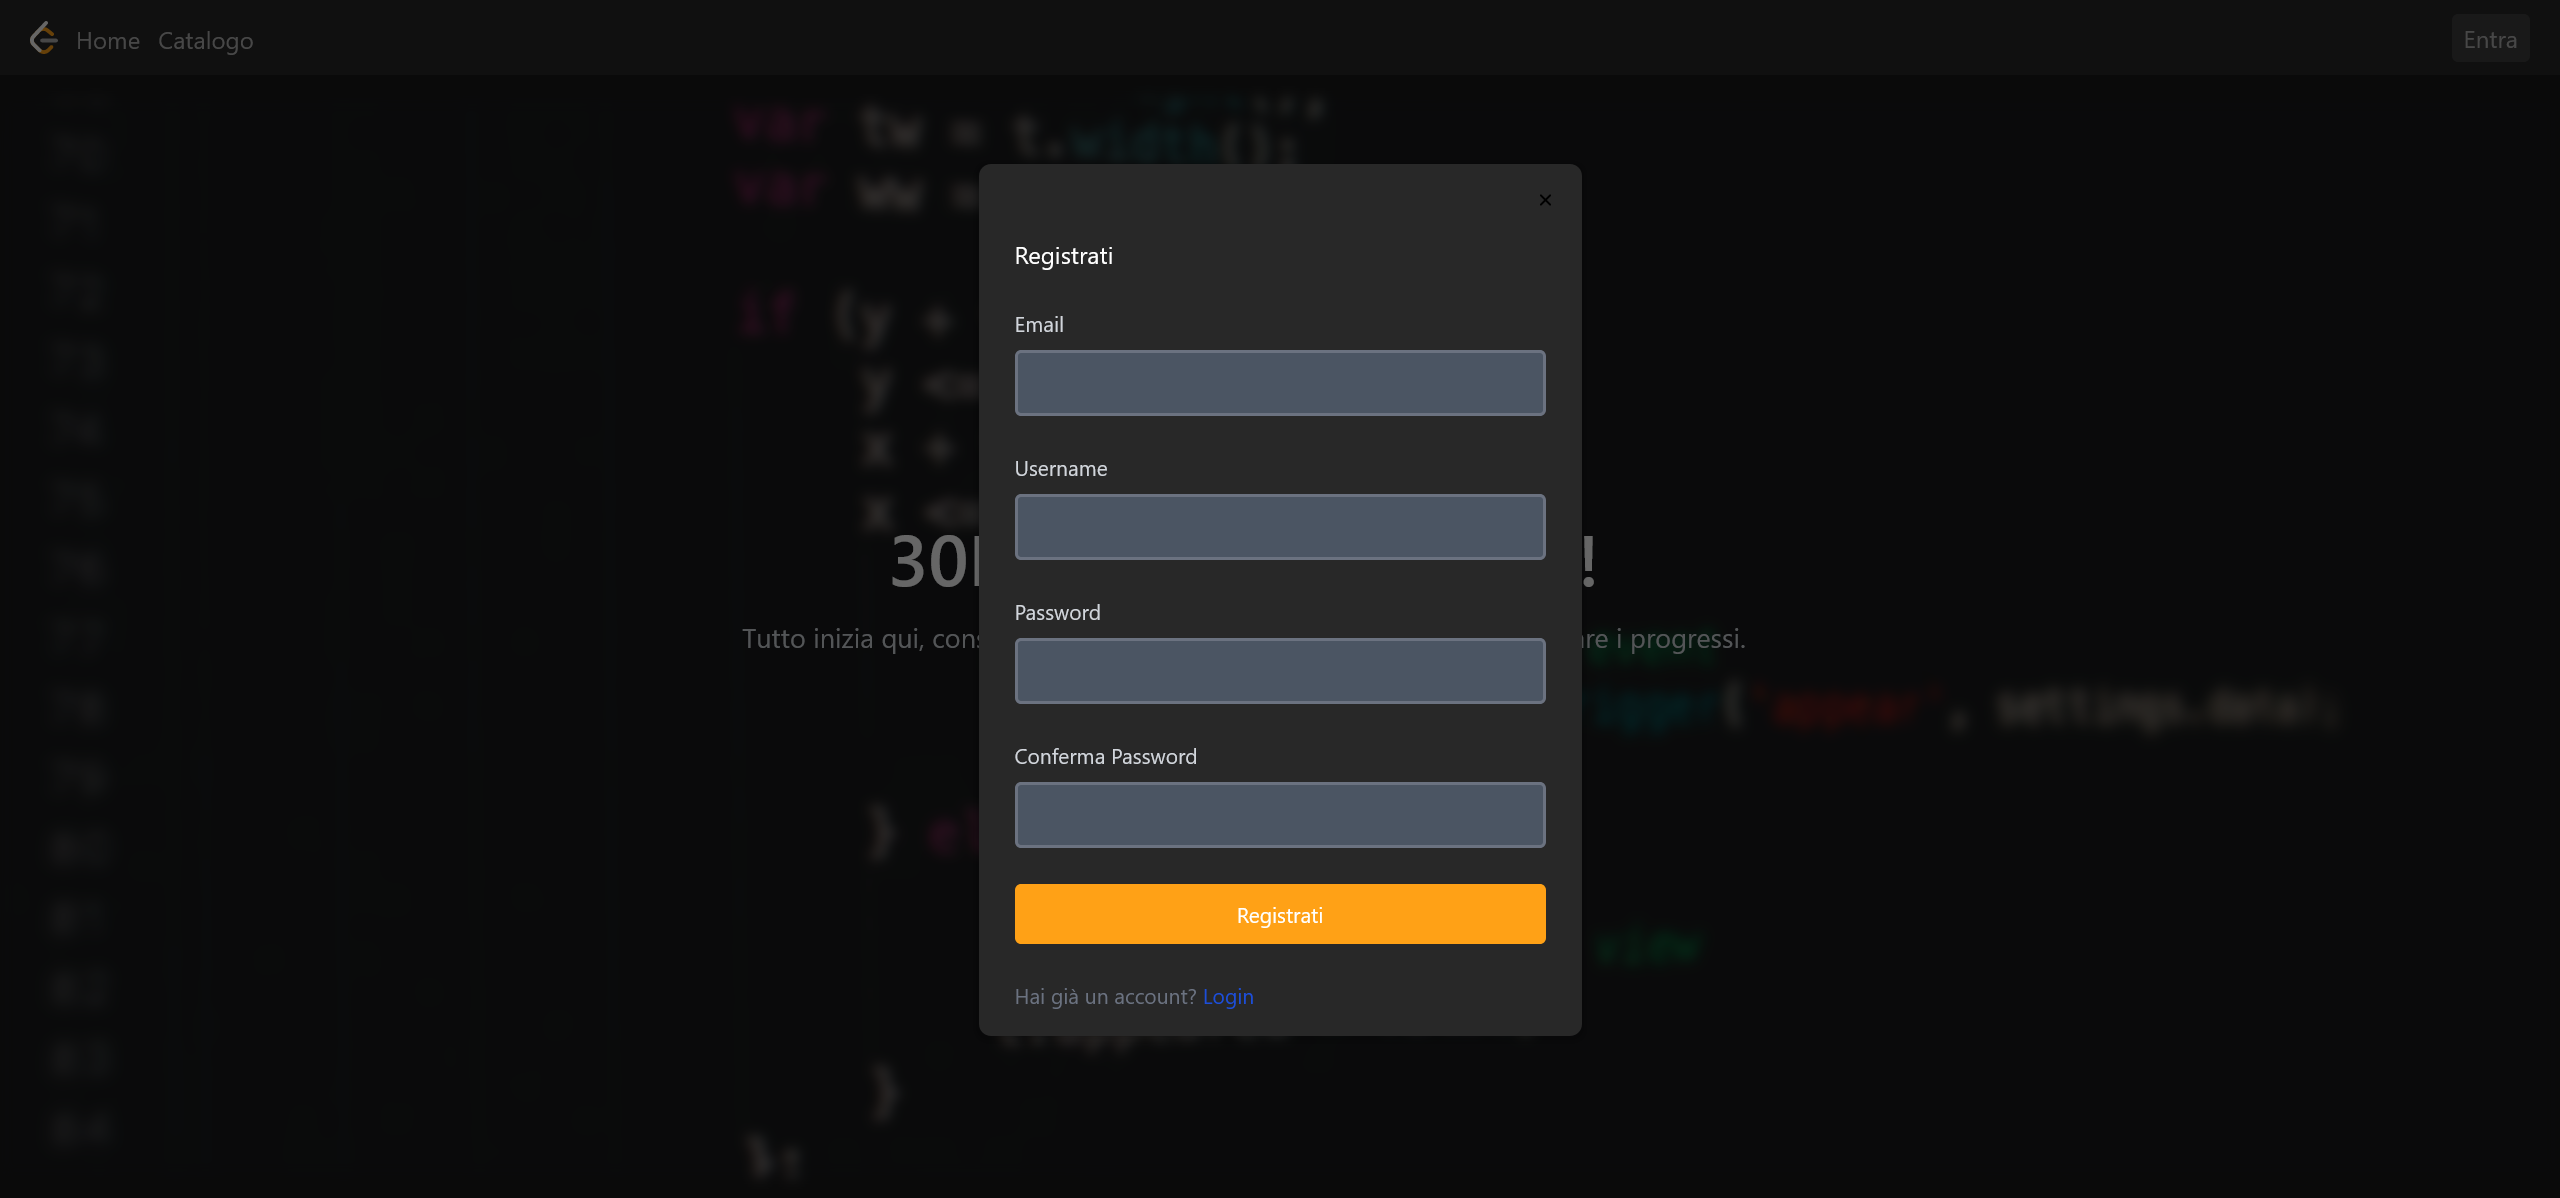
\includegraphics[width=\textwidth]{materiale/sito/Signup.png}
\end{figure}

\subsection{Recupero Password}
Questo componente permette ad un utente non ancora autenticato di richiedere una mail per recupero password, anche se la mail non è registrata verrà comunque dato un messaggio di conferma di invio, per ragioni di sicurezza. Come già scritto precedentemente
a causa di limitazioni col piano Firebase non possiamo impostare regole per le password "recuperate" in quanto gestite da componenti interni di Firebase non disponibili al nostro piano gratuito.\\\\

\begin{figure}[H]
  \centering
  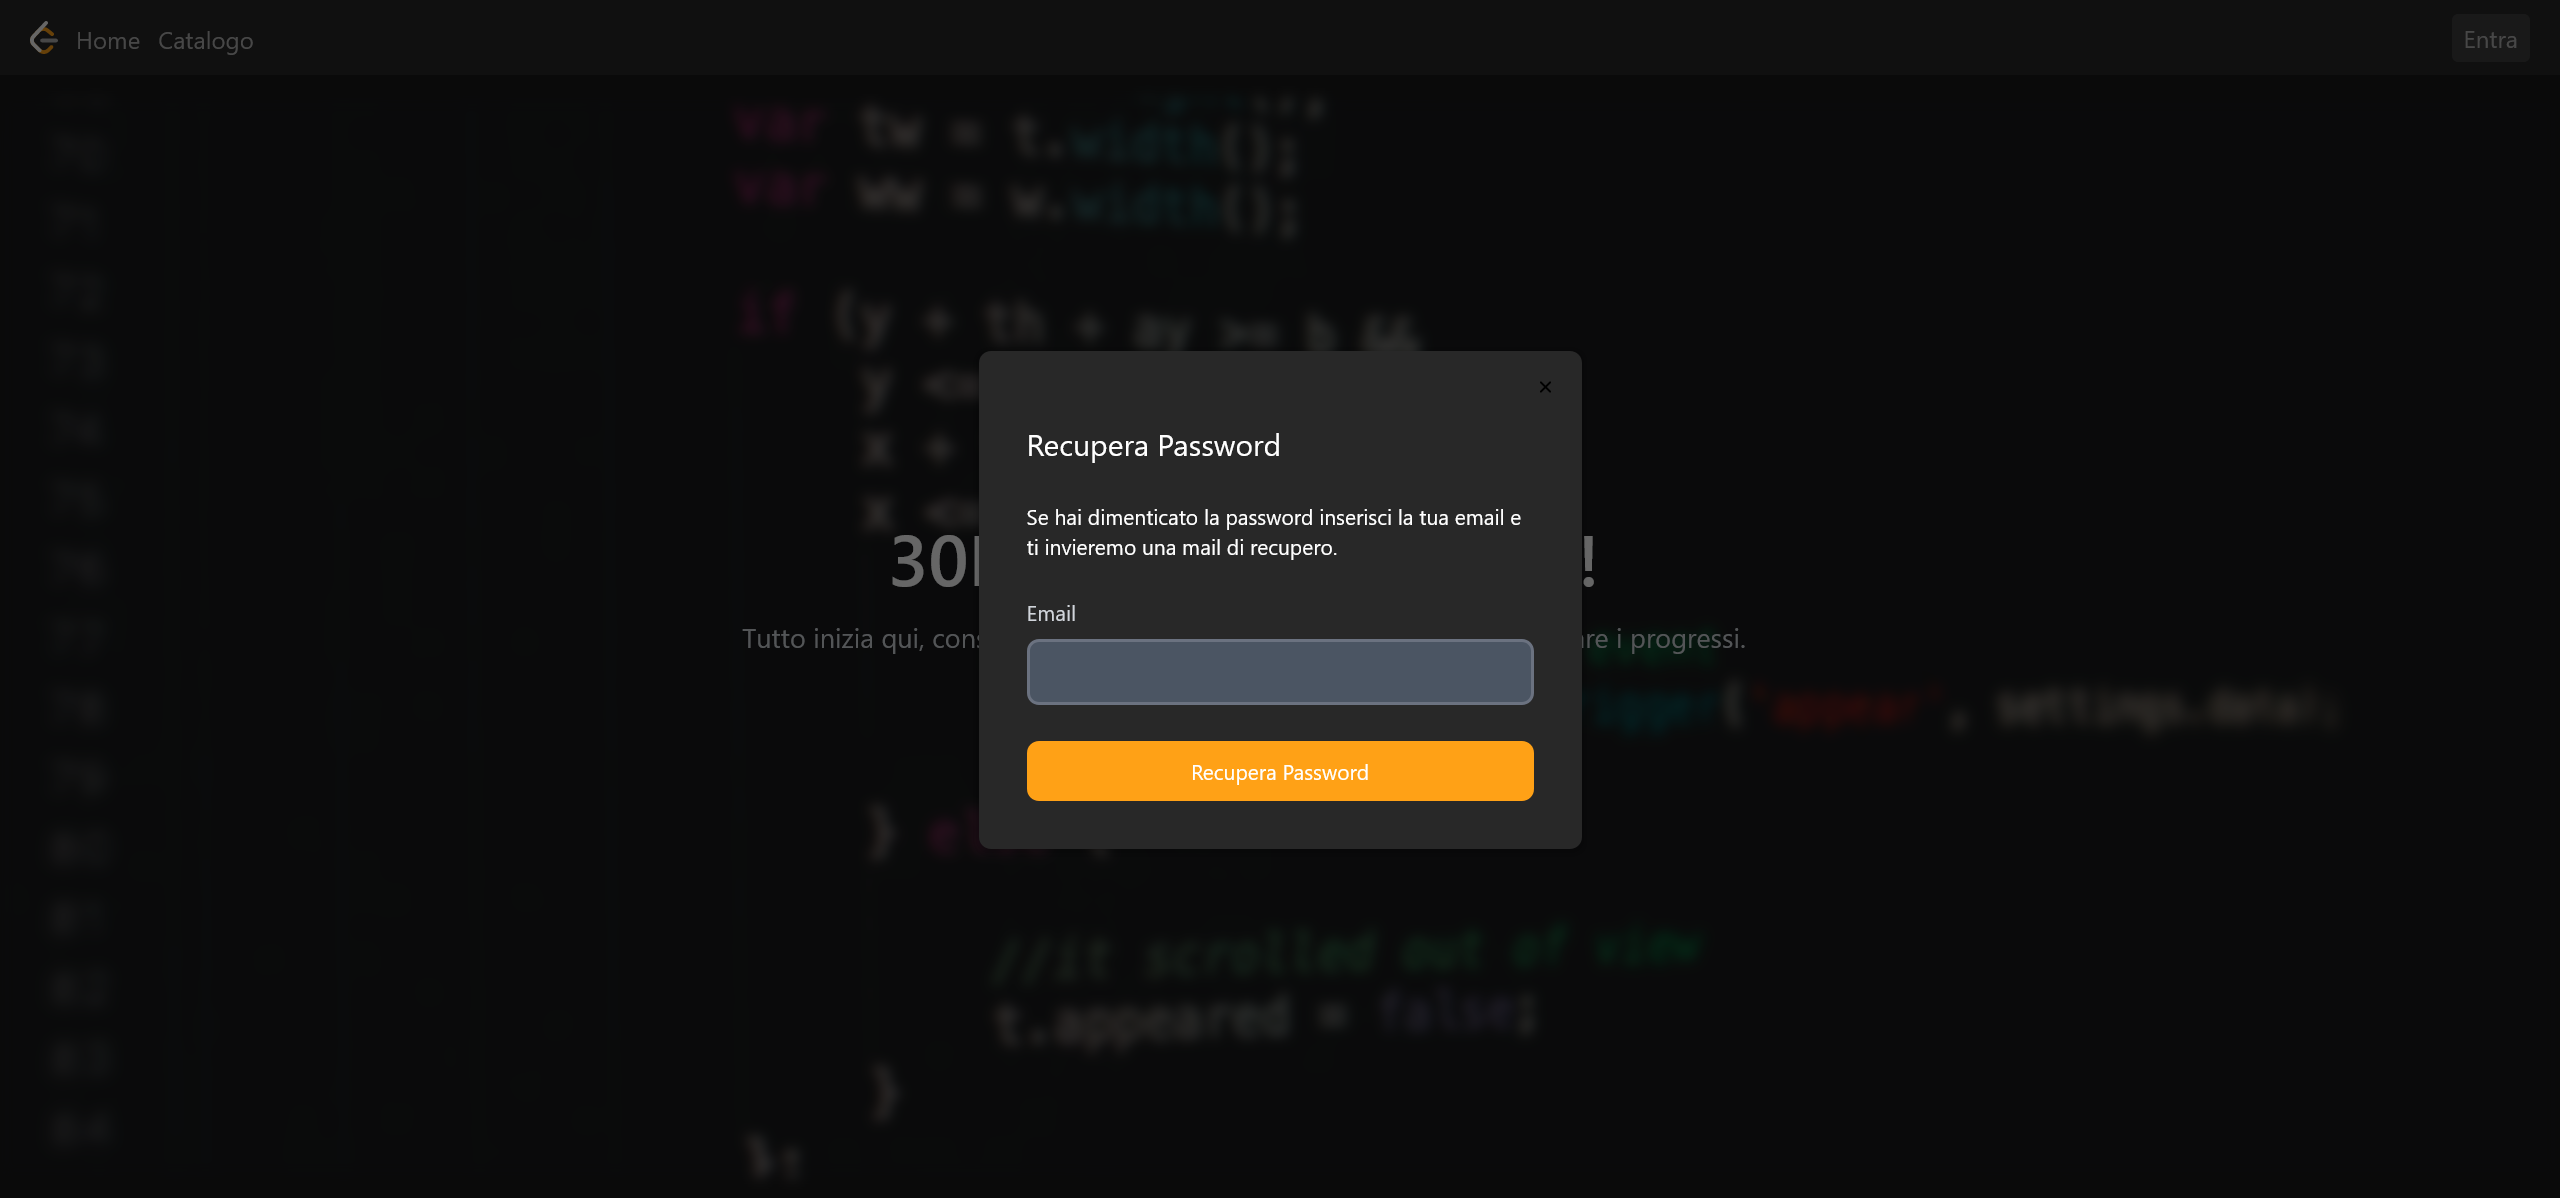
\includegraphics[width=\textwidth]{materiale/sito/Recupero Pw.png}
\end{figure}

\subsection{Pannello Admin}
Questo componente (non completamente sviluppato) permette ad un utente amministratore di aggiungere problemi al database.

\begin{figure}[H]
  \centering
  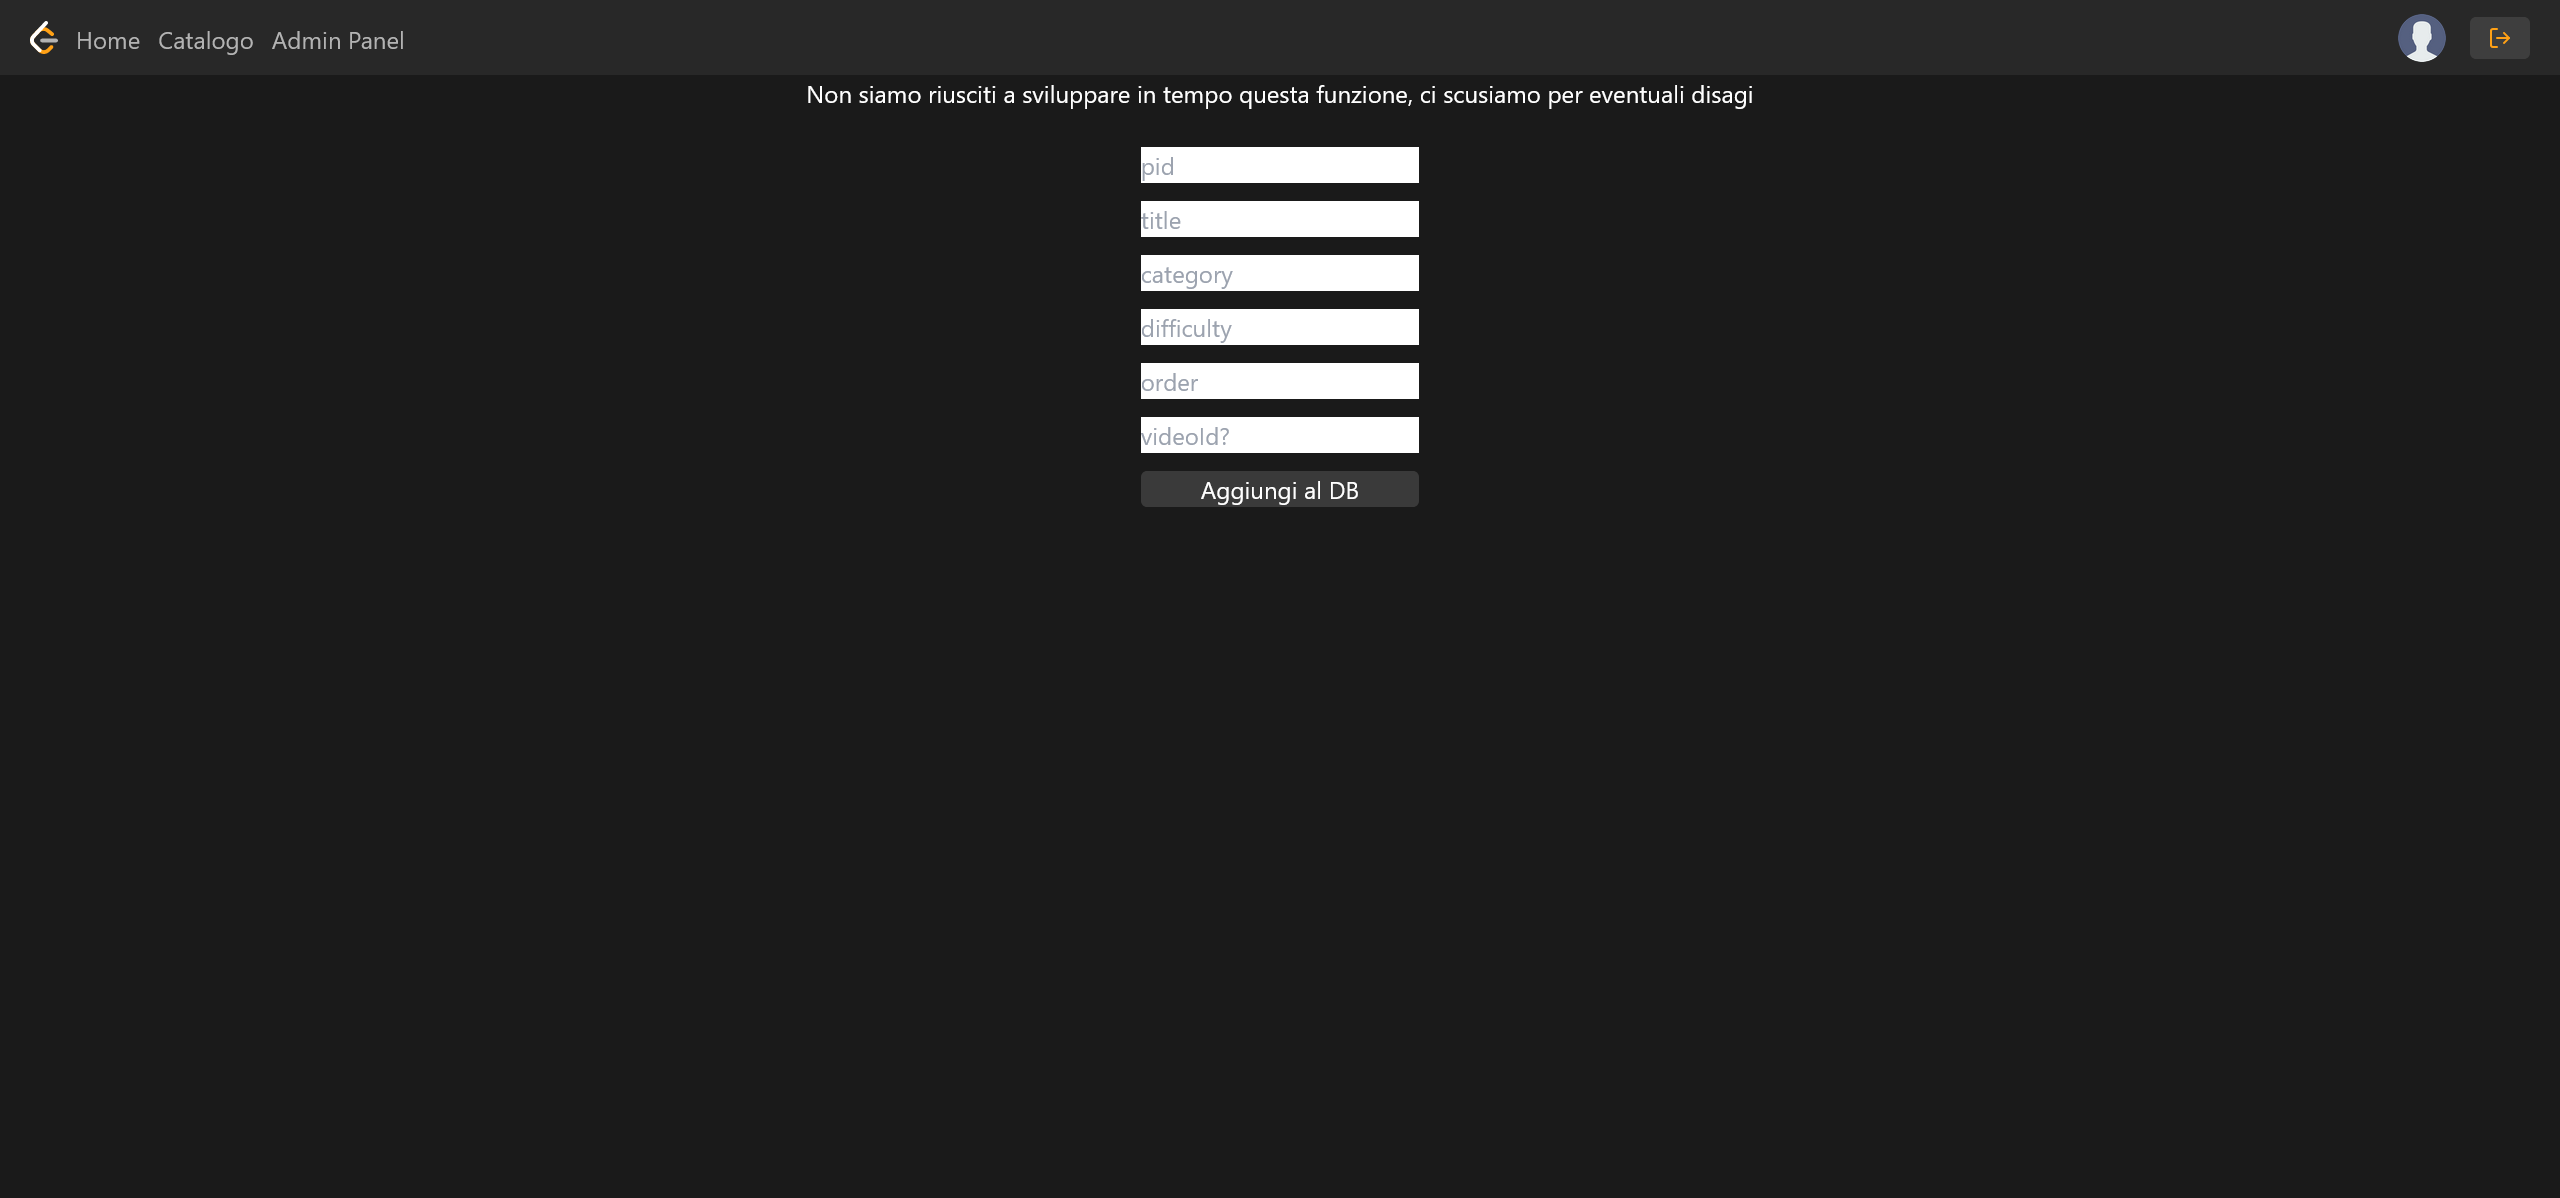
\includegraphics[width=\textwidth]{materiale/sito/Pannello Admin.png}
\end{figure}

\subsection{Pagina Profilo}
Questa pagina permette ad un utente autenticato di accedere alle funzioni di modifica password e di eliminazione account attraverso appositi form, in caso un utente cerca di accedersi senza essere autenticato verrà riportato alla home.\\\\

\begin{figure}[H]
  \centering
  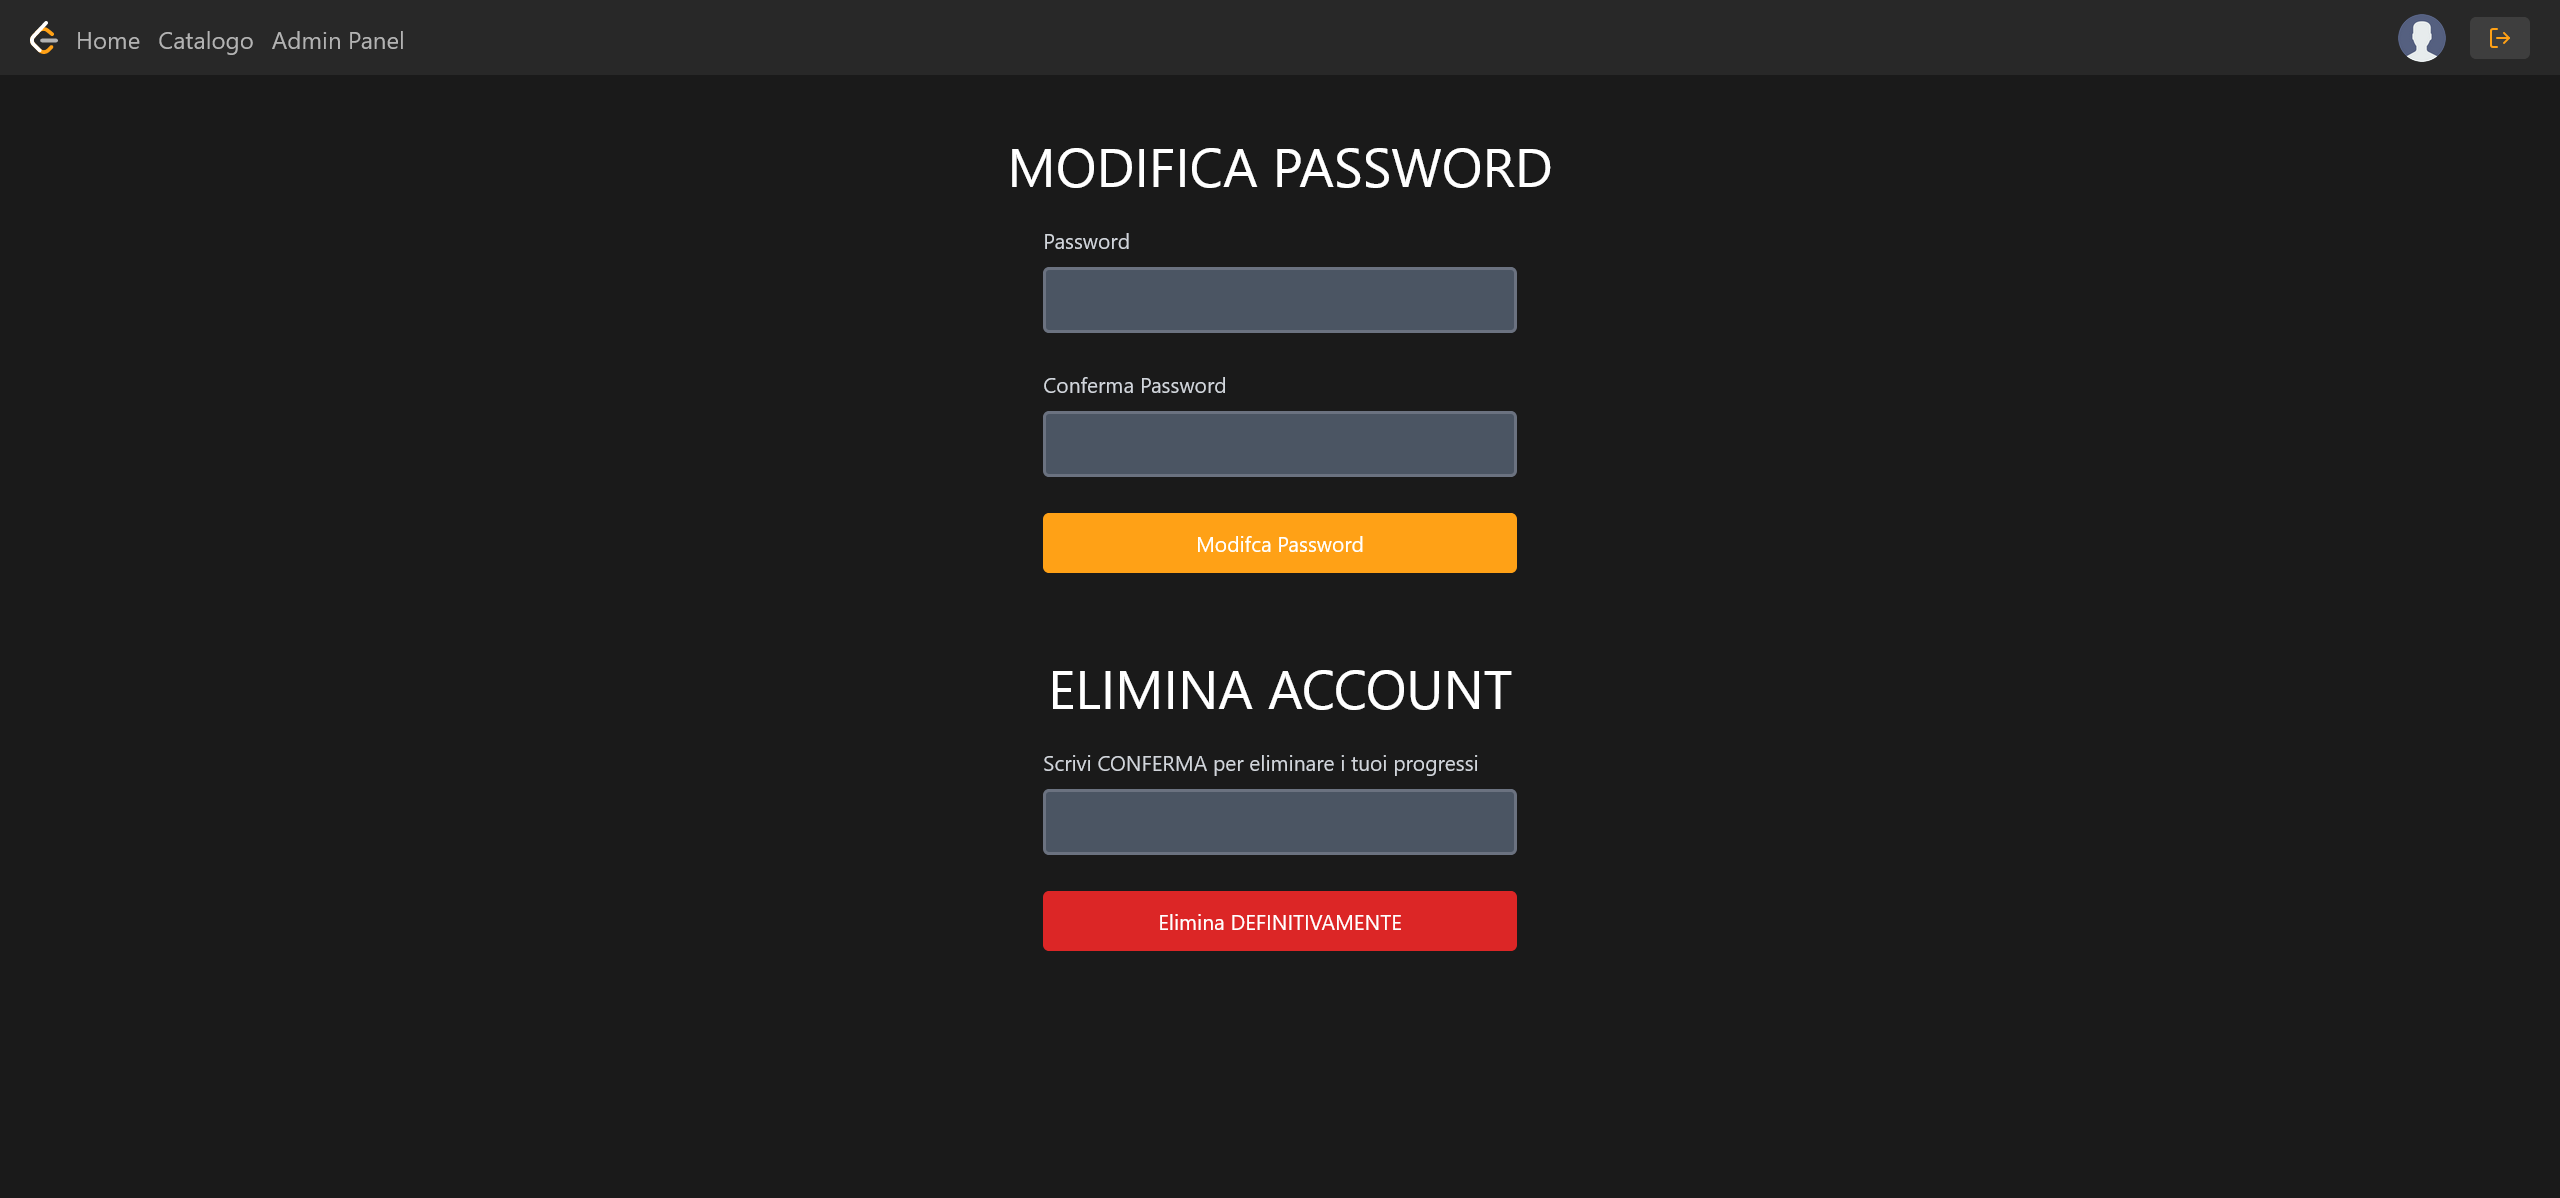
\includegraphics[width=\textwidth]{materiale/sito/Pagina Profilo.png}
\end{figure}

\subsection{Catalogo}
Questa pagina raccoglie tutti i problemi disponibili, la loro difficoltà, categoria
ordine, titolo e videoId, e gli offre a tutti gli utenti, in caso l'utente sia autenticato, verrà mostrato un componente
 che traccia i progressi del singolo utente, e i problemi risolto e/o aggiunti ai preferiti. Oltre a questo un qualsiasi
utente cliccando sull'icona nella colonna "\textbf{Soluzione}" verrà aperta una overlay per visualizzare un video che offre suggerimenti su come risolvere il problema e la soluzione in linguaggio Javascript.
Quando un qualsiasi utente si connette verrano mostrati degli "Scheletri" per mostrare all'utente che la pagina sta aspettando informazioni dal server, e che di conseguenza dovrà aspettare.\\\\

\begin{figure}[H]
  \centering
  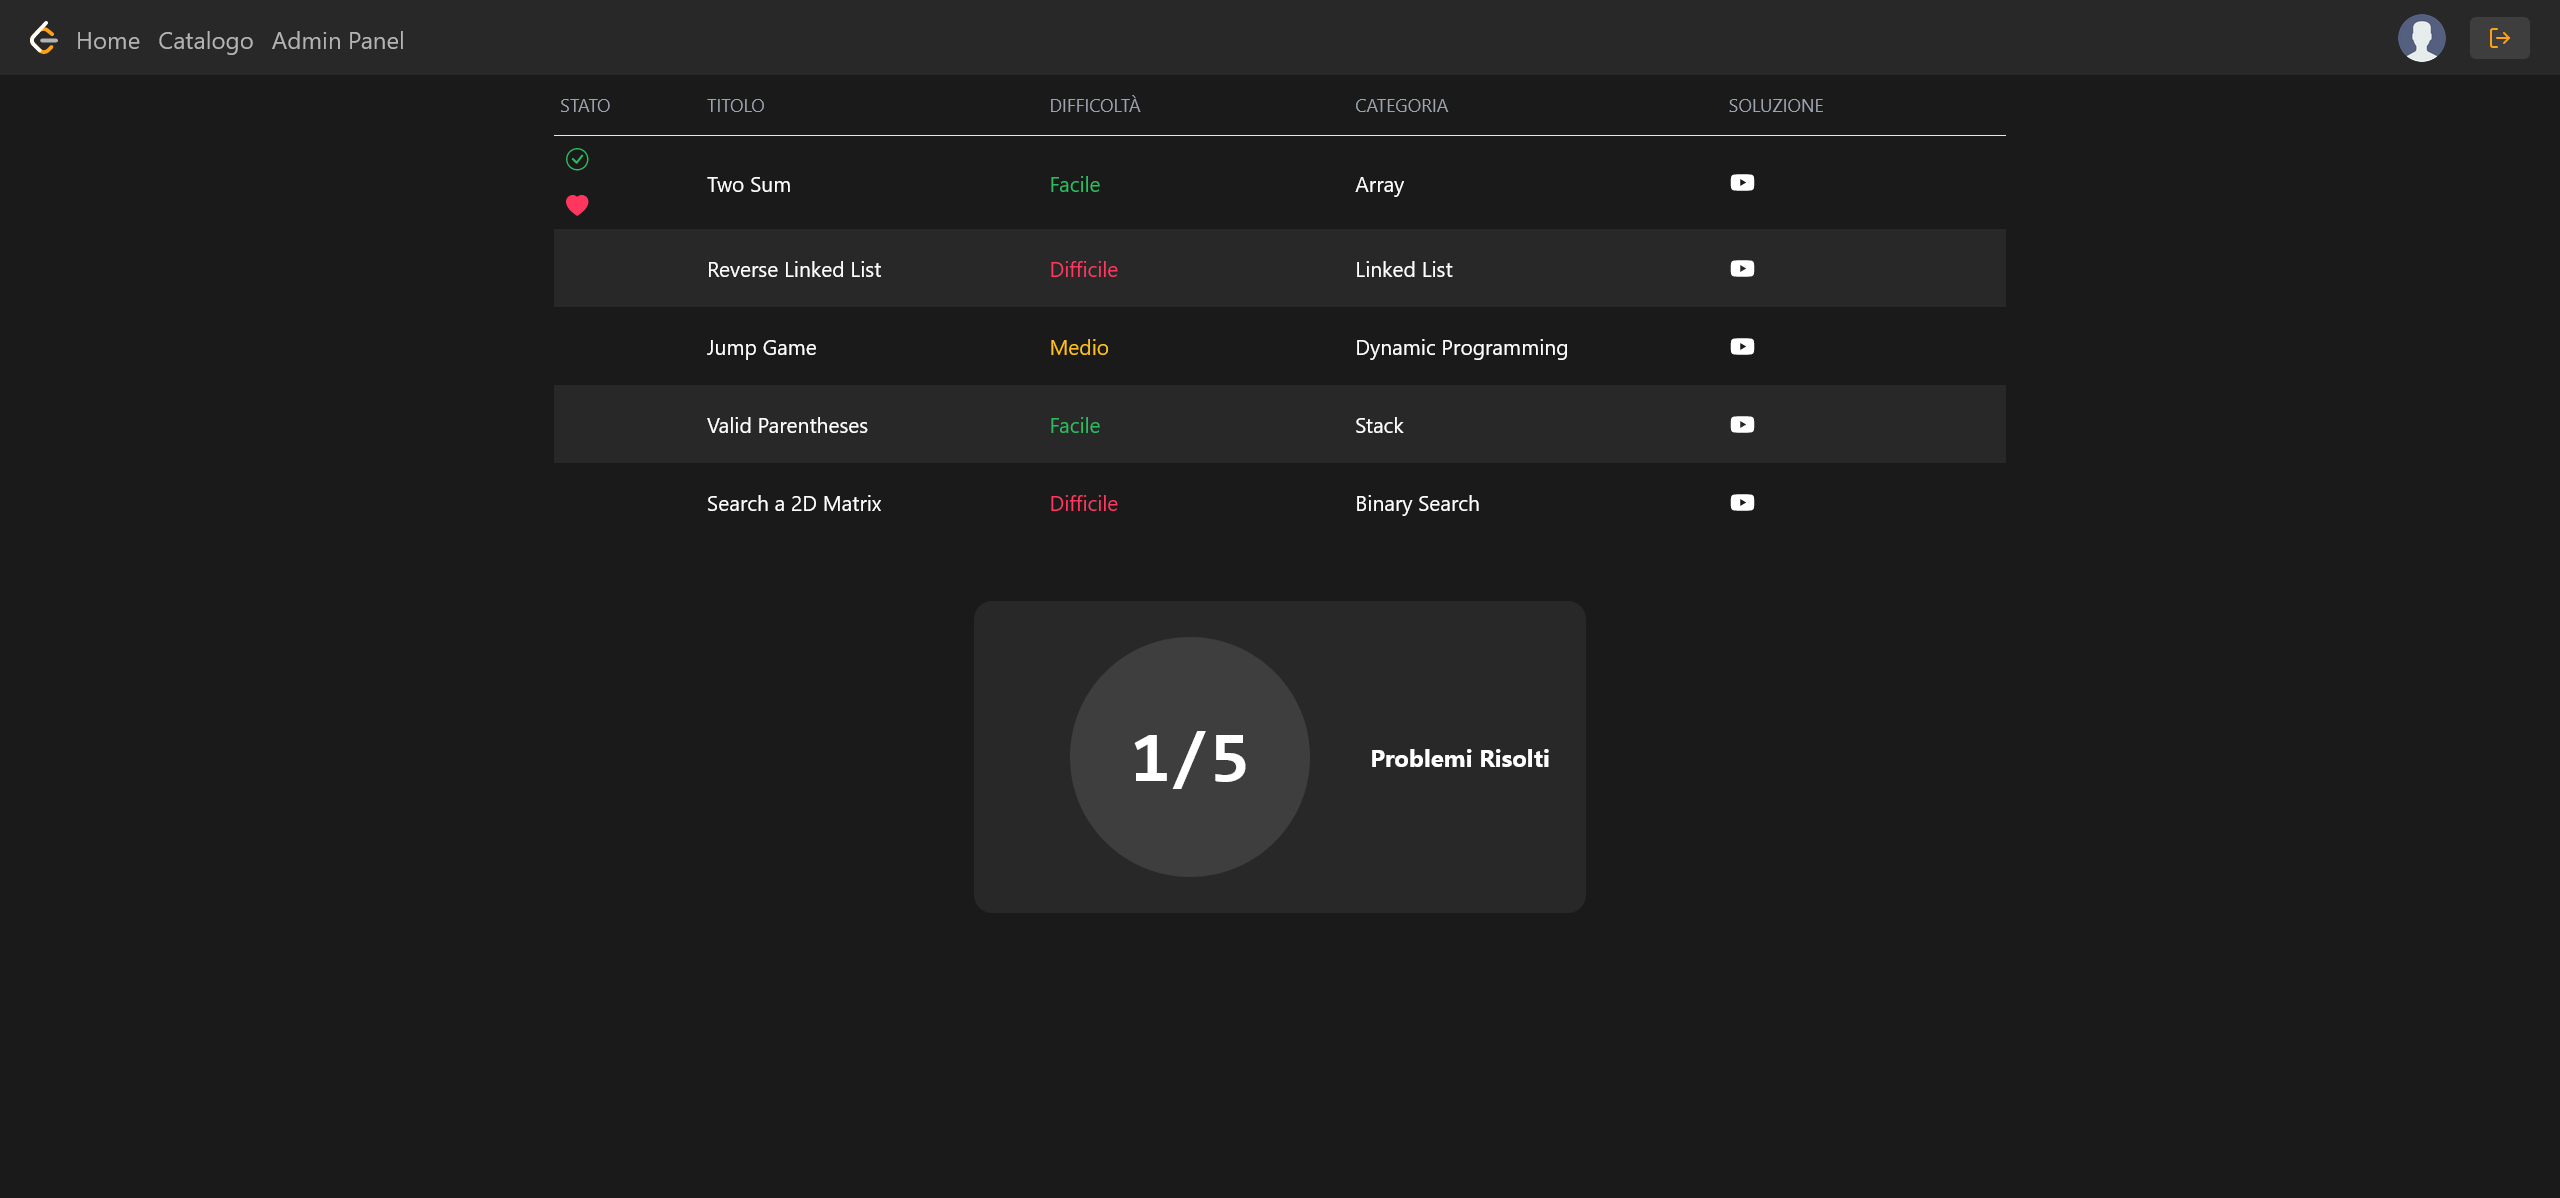
\includegraphics[width=\textwidth]{materiale/sito/Catalogo.png}
\end{figure}

\subsection{Area di esercitazione}
Questa pagina esiste per ogni problema al momento disponibile ed è suddivisa in 3 parti:
\begin{itemize}
  \item Descrizione: Contiene tutte le informazioni e/o immagini relative al problema, oltre ad indicaticare e permettere di aggiungere un problema ai preferiti e visualizzare il numero di "like" e capire se il problema è gia stato risolto. Oltre a questo abbiamo un numero variabile di esempi per aiutare l'utente nella risoluzione del problema.
  \item Console: Dove l'utente può scrivere codice e selezionare il linguaggio con cui risolvere il problema. Al momento della realizzazione del progetto, l'unico linguaggio disponibile è Javascript, siccome altri linguaggi richiederebbero server dedicati per la compilazione del file. Ricordiamo di non modificare la firma della funzione.
  \item Testcase: Dove l'utente è in grado di selezione quale test case vedere e sottomettere o provare a risolvere il problema attraverso appositi bottoni. (\textbf{Sottometti o Runna})
\end{itemize}
Oltre a questo ogni utente (anche non autenticato) è in grado di cliccare sull'icona a forma di orologio e cronometrare il proprio tempo di risoluzione del problema, il fermare o resettare il cronometro è compito dell'utente.
\\\\
In caso l'utente connesso alla pagina non dovesse essere autenticato, egli non potrà tracciare i propri progressi, né aggiungere problemi ai preferiti; in caso si tenti di eseguire quest'ultima azione, verrà riportato un messaggio di errore.
\\\\


\begin{figure}[H]
  \centering
  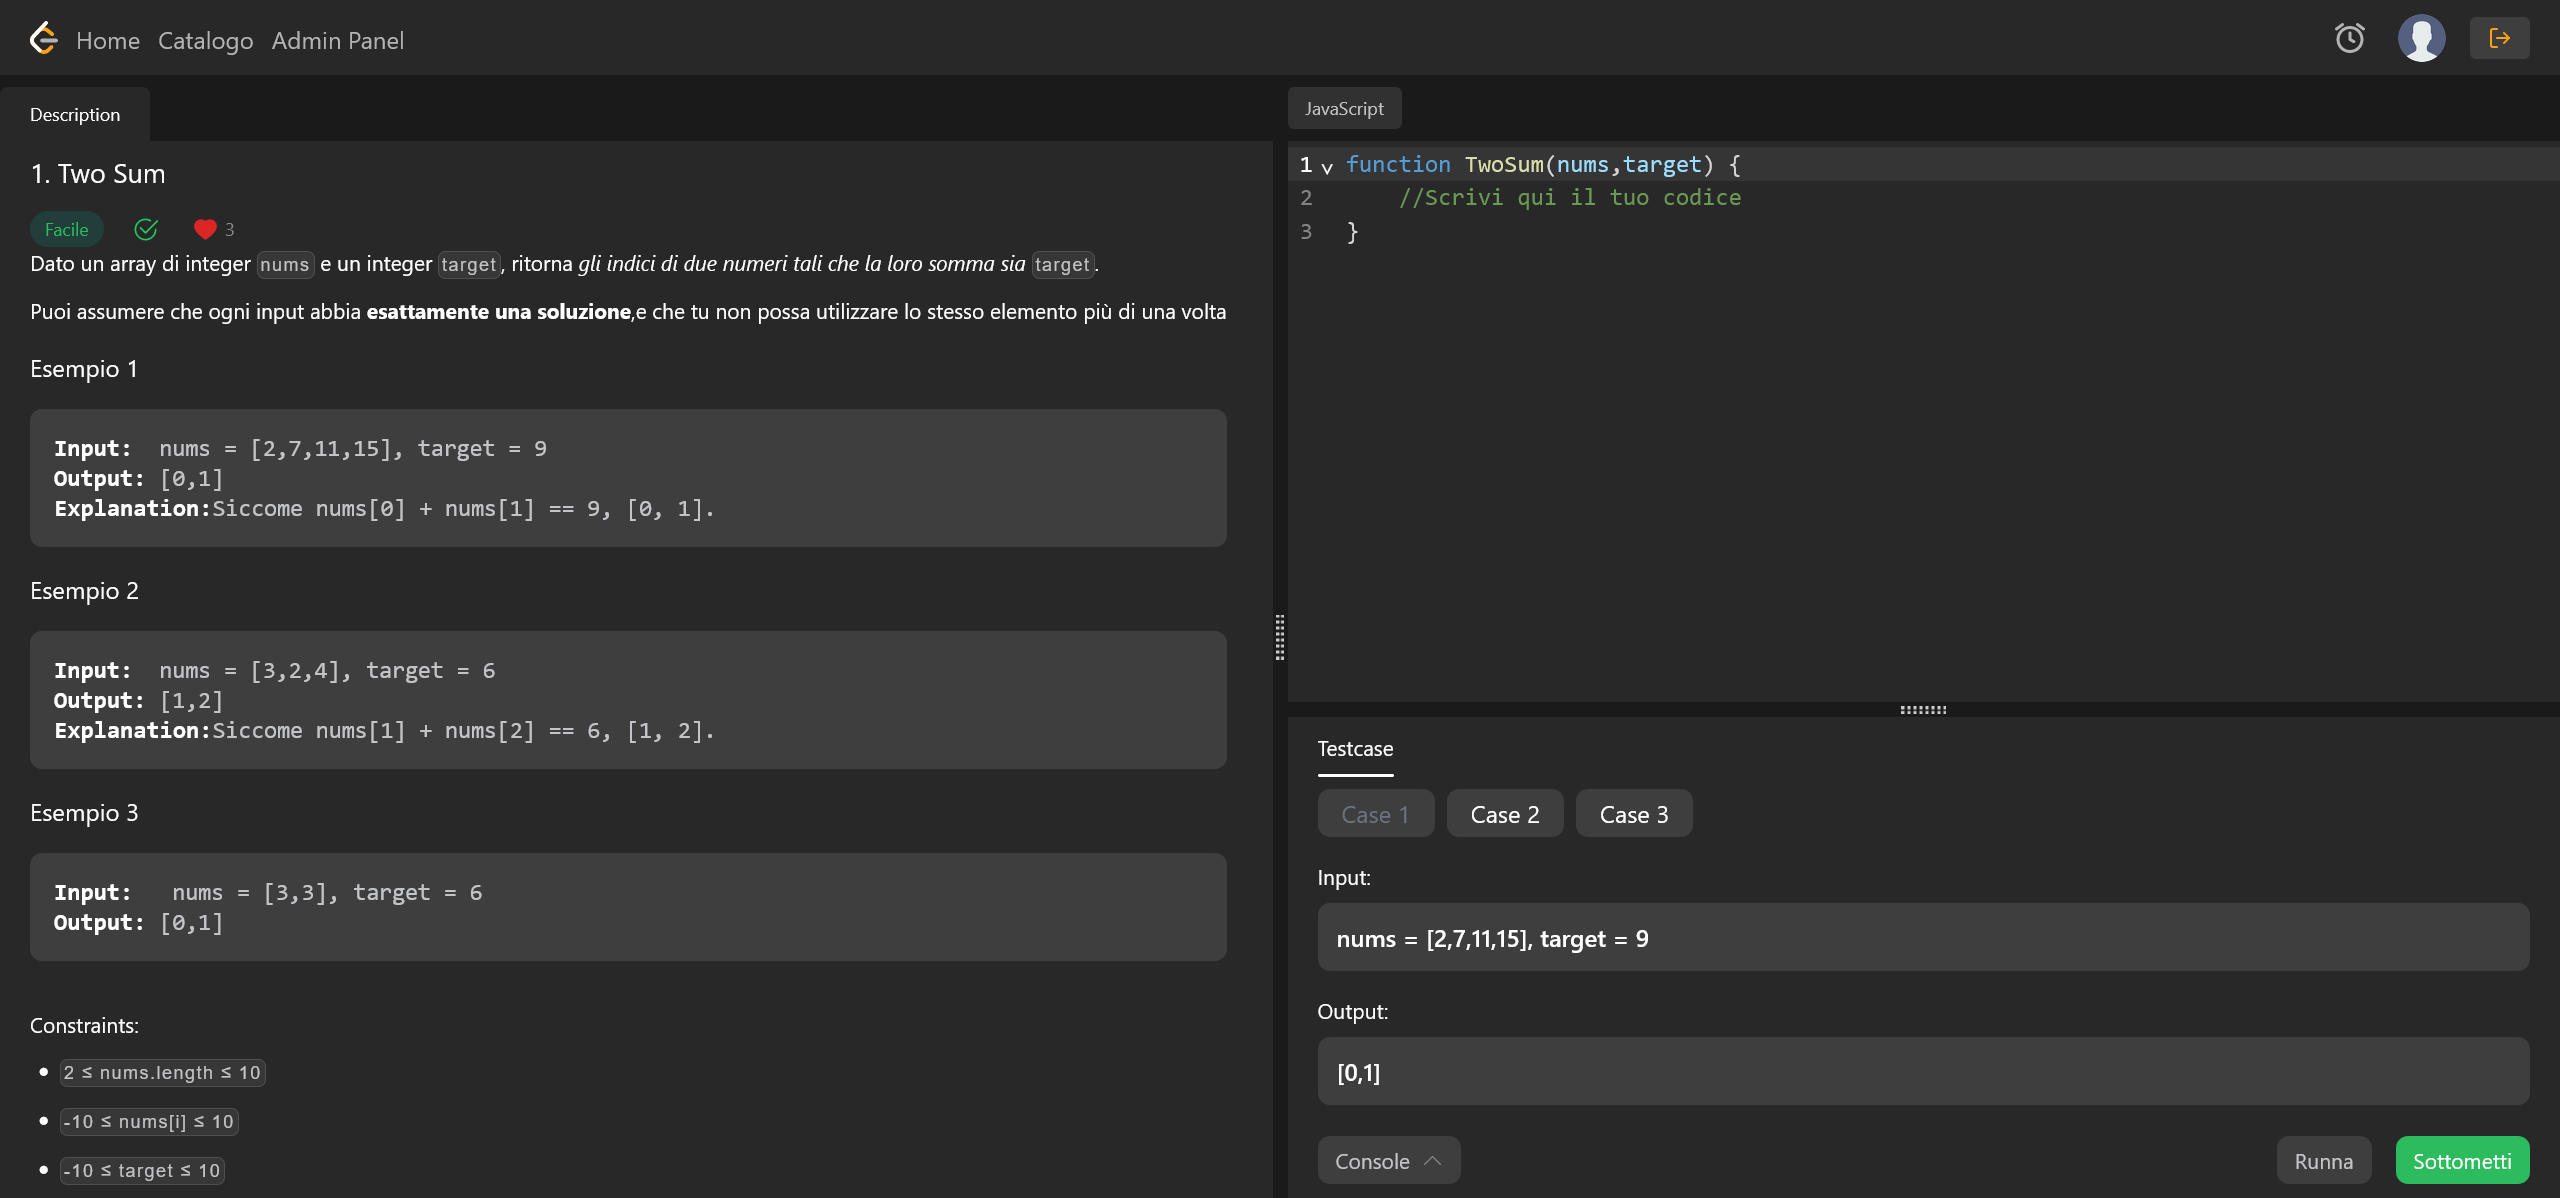
\includegraphics[width=\textwidth]{materiale/sito/Problema.png}
\end{figure}

\newpage
\section{Github Repository \& Deployment Information}
La repositories del progetto sono disponibili all'interno dell'organizzazione
G17-UniTn su GitHub, al seguente link:
\begin{center}
  \href{https://github.com/G17-UniTn}{G17-UniTn}
\end{center}
L'organizzazione è suddivisa in tre repositories:
\begin{itemize}
  \item \textbf{Deliverables}: contiene tutte le risorse impiegate per realizzare in \LaTeX\texttt{ } i documenti D1, D2, D3, D4 e D5, inclusi i file \texttt{.pdf}, i sorgenti \texttt{.tex} e le immagini.
  \item \textbf{Documents}: raccoglie solamente i file PDF dei cinque deliverables, identici a quelli presenti in Deliverables e a quelli consegnati al termine del progetto.
  \item \textbf{CodeBase}: contiene tutto il codice relativo al front-end ed al back-end.
\end{itemize}
Il gruppo che ha sviluppato il progetto all'interno dell'organizzazione G17-UniTn, sul sito GitHub, è composto dai seguenti membri:
\begin{itemize}
  \item Raffaele Castagna \href{https://github.com/Raffaele-Castagna}{\textcolor{black}{\faGithub}}
  \item Zeno Saletti \href{https://github.com/zenosalty}{\textcolor{black}{\faGithub}}
  \item Alberto Rovesti \href{https://github.com/uniBeto}{\textcolor{black}{\faGithub}}
\end{itemize}
Il sito è attualmente attivo ed hostato sulla piattaforma Vercel. Di seguito è riportato il link per visualizzare il sito web:
\begin{center}
  \url{https://sleepcode-dev.vercel.app/}
\end{center}
Per poter testare il sito a livello di accesso amministratore, è stato creato un account che gode dei privilegi di amministratore:

\begin{center}
  Email: \texttt{admin@gmail.com}, password: \texttt{PasswordAdmin2024!}
\end{center}
Per testare agevolmente il funzionamento dei test cases, viene fornito
in CodeBase il file
\begin{center}
  \href{https://github.com/G17-UniTn/CodeBase/blob/master/SOLUZIONI.txt}{\texttt{soluzioni.txt}}
\end{center}
contenente algoritmi corretti per risolvere tutti i problemi
presenti nel catalogo al momento del completamento del progetto (è sufficiente
copiare e incollare i codici nella console dell'area di esercitazione).


\newpage
\section{Testing}
Per eseguire il testing, è stato utilizzato il pacchetto \href{https://jestjs.io/}{Jest} ed è stato inoltre integrato con Firebase con il pacchetto \href{https://www.npmjs.com/package/firestore-jest-mock}{Jest-firestore-mock}. Per simulare le richieste API sono stati
utilizzati i pacchetti \href{https://www.npmjs.com/package/node-mocks-http}{node-mocks-http}.\\
Sono state definite due cartelle \href{https://github.com/G17-UniTn/CodeBase/tree/master/__mocks__}{\_\_mocks\_\_} e \href{https://github.com/G17-UniTn/CodeBase/tree/master/__test__}{\_\_test\_\_}: la prima è stata creata per utilizzare le funzioni di ``mock" di Jest 
che permettono a quest'ultimo di ``imitare" connessioni al database e/o credenziali, molto utile nel testing di API che richiedono funzioni disponibili solo alla \href{https://firebase.google.com/docs/reference/admin}{SDK admin} di firebase.
\\\\
Di seguito riportiamo le diverse test suite create

\begin{figure}[H]
  \centering
  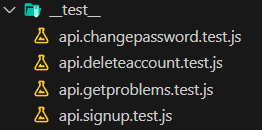
\includegraphics[scale = 1]{materiale/testing/test-overview.png}
\end{figure}

\subsection{Test API}
Di seguito sono mostrati i risultati delle test suite applicate sulle diverse API.

\subsubsection{test api/signup}
\begin{figure}[H]
  \centering
  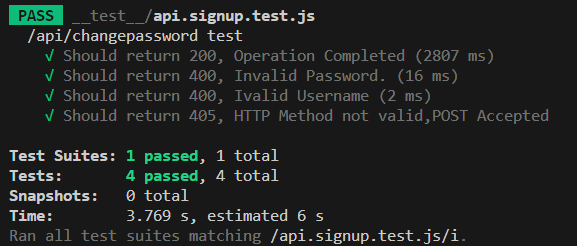
\includegraphics[scale = 1.1]{materiale/testing/Signup.png}
\end{figure}

\subsubsection{test api/changepassword}
\begin{figure}[H]
  \centering
  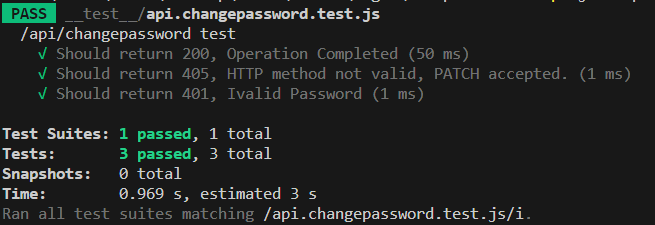
\includegraphics[width = \textwidth]{materiale/testing/ChangePw.png}
\end{figure}

\subsubsection{test api/deleteAccount}
\begin{figure}[H]
  \centering
  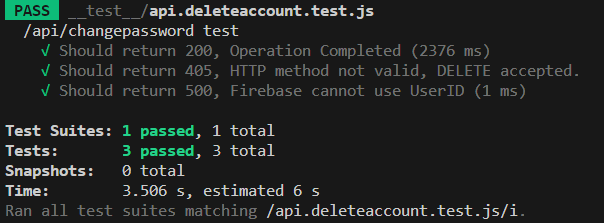
\includegraphics[width = \textwidth]{materiale/testing/DeleteAccount.png}
\end{figure}

\subsubsection{test api/getProblems}

\begin{figure}[H]
  \centering
  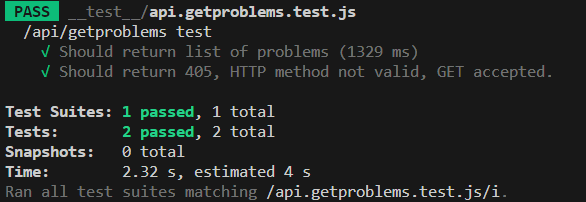
\includegraphics[width = \textwidth]{materiale/testing/GetProblems.png}
\end{figure}

\newpage
\subsection{Code Coverage}
Di seguito riportiamo il code coverage generato da Jest.
\begin{figure}[H]
  \centering
  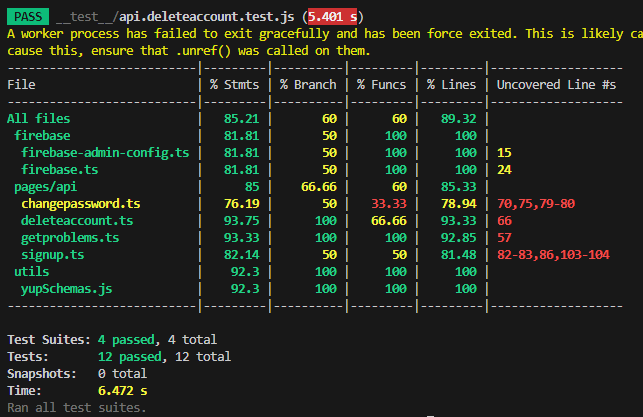
\includegraphics[scale = 1]{materiale/testing/Code Coverage.png}
\end{figure}

\end{document}